\documentclass{article}
\usepackage{graphicx}
\usepackage{float}
\graphicspath{{Illustrations/}}

\title{\textbf{COMP1044 Coursework Assignment 2 Report B} \\ Group 15 / Chew Language}
\author{
	Leong Chang Yung, 20307078
	\and
	Lucas Dylan Purnell, 20197316
	\and
	Tan Zhun Xian, 20313854
	\and
	Chong Hao Wei, 20194465
	\and
	Morhaf Allababidi, 20195867
	\and
	Thomas Tan Kean Yew, 20316601
}
\date{\today}

\begin{document}
\maketitle
\newpage

\section{Entity Relation Diagram}
	\begin{figure}[h!]
		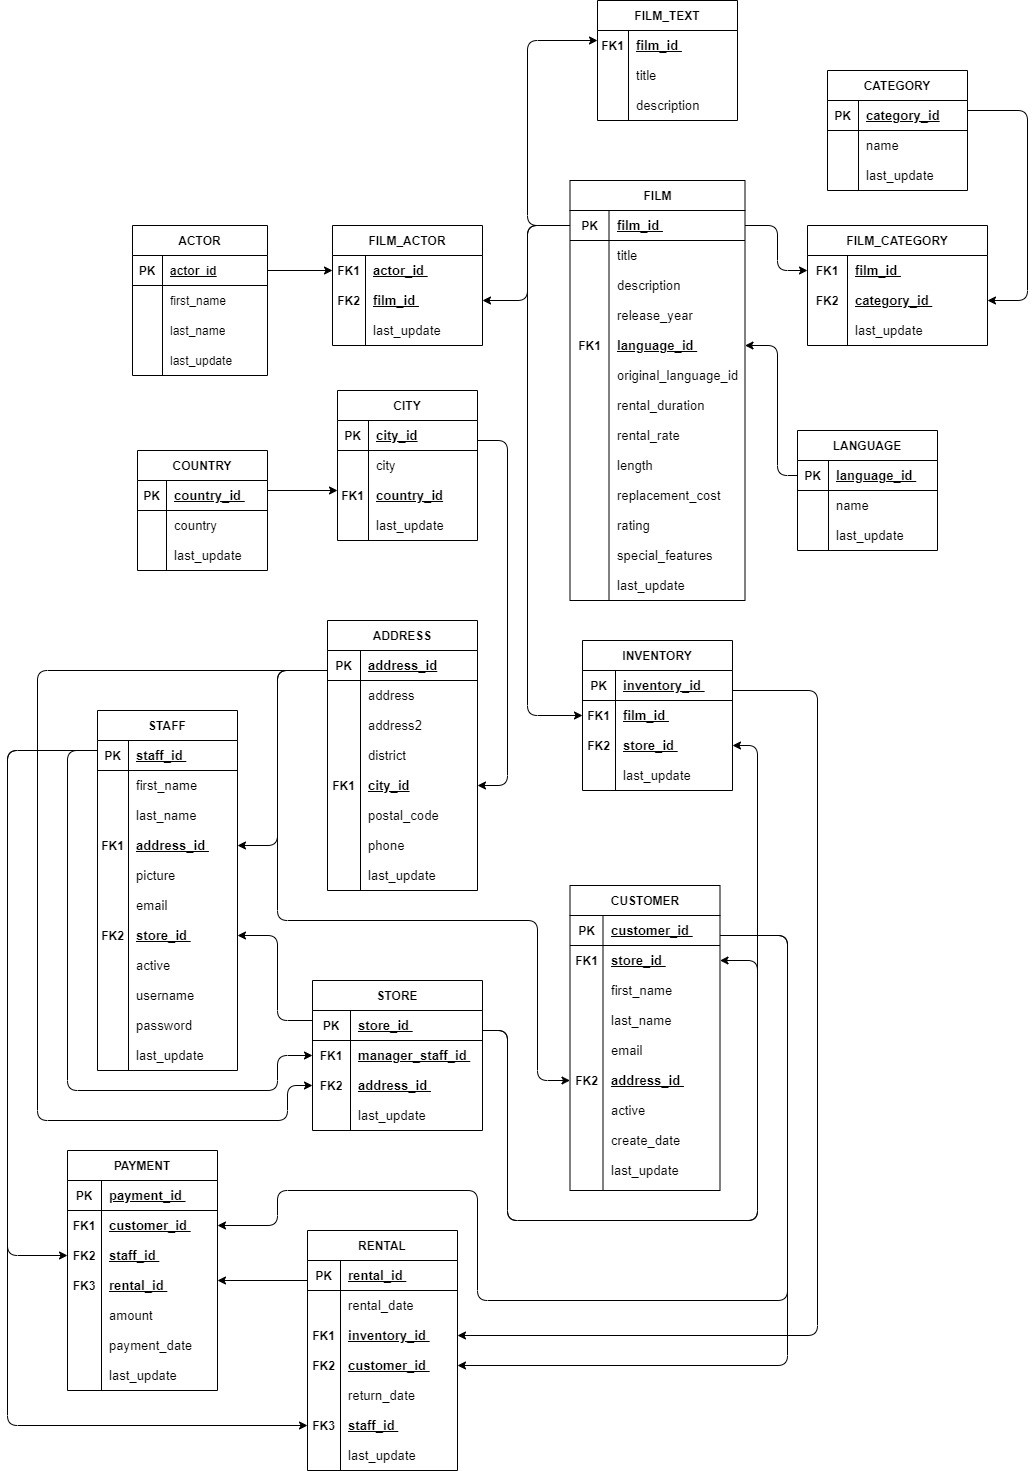
\includegraphics[height=.8\textheight, width=\textwidth]{er_diagram}
		\caption{Proposed Entity Relation Diagram arrangement. \protect\footnotemark}	
	\end{figure}
	\footnotetext{This diagram is based on available table data provided.}


\section{Database Creation}
	\begin{figure}[H]
		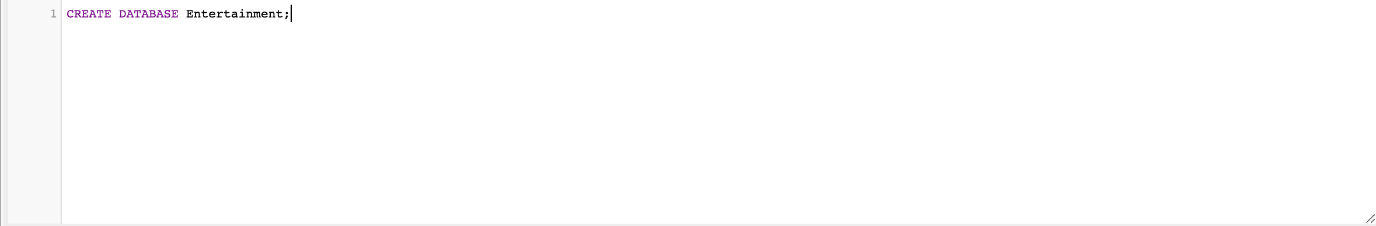
\includegraphics[width=\textwidth]{database_create}
		\caption{Creation of database "Entertainment"}	
	\end{figure}
	\rule{\textwidth}{0.4pt}
\section{Creation and Insertion of Tables}
	\begin{figure}[H]
		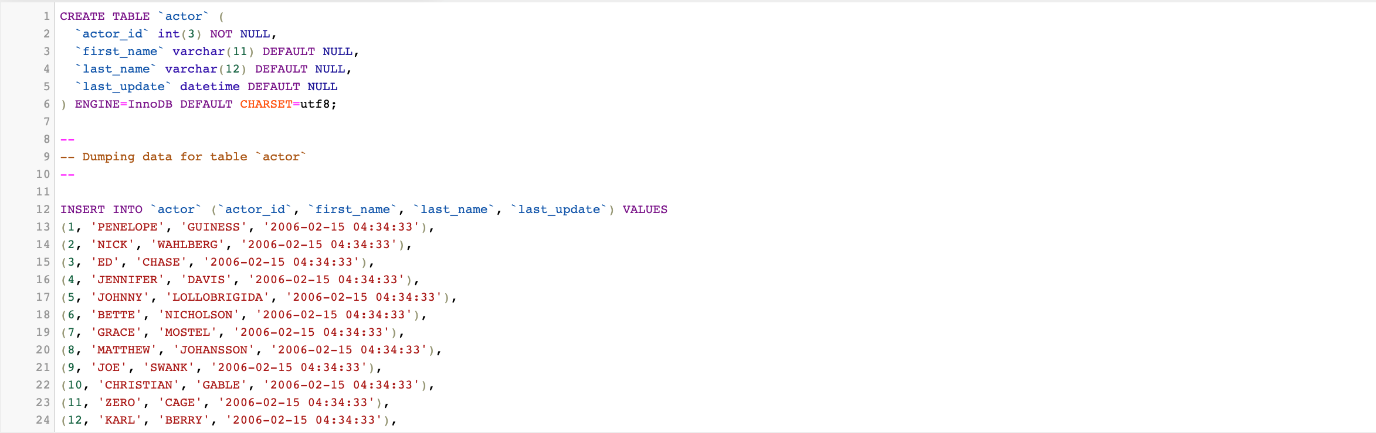
\includegraphics[width=\textwidth]{table_actor_cins}
		\caption{Creation and Insertion of table "Actor"}	
	\end{figure}
	\begin{figure}[H]
		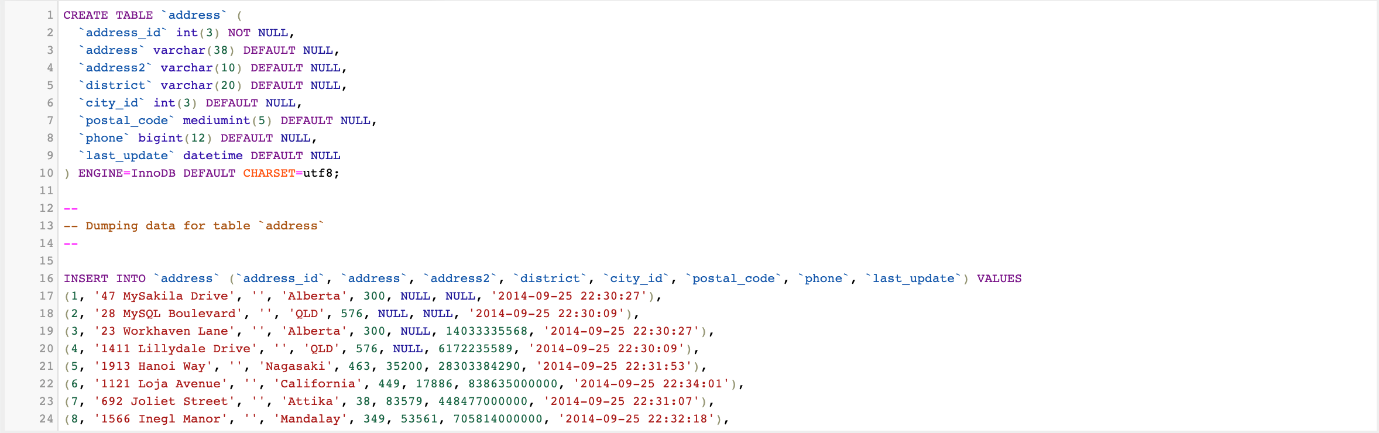
\includegraphics[width=\textwidth]{table_address_cins}
		\caption{Creation and Insertion of table "Address"}	
	\end{figure}
	\begin{figure}[H]
		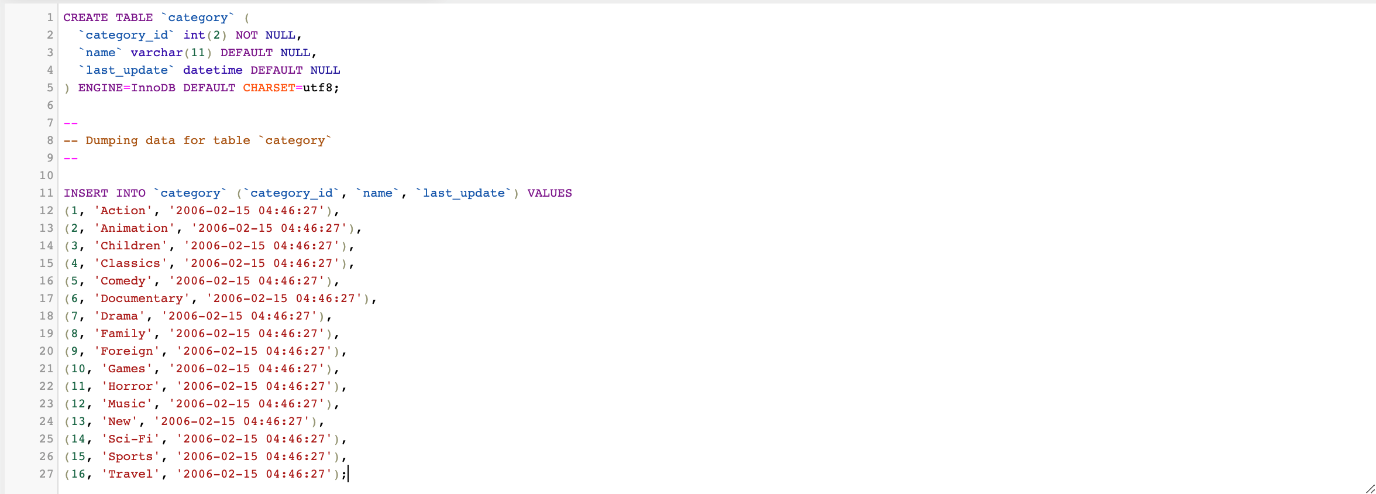
\includegraphics[width=\textwidth]{table_category_cins}
		\caption{Creation and Insertion of table "Category"}	
	\end{figure}
	\begin{figure}[H]
		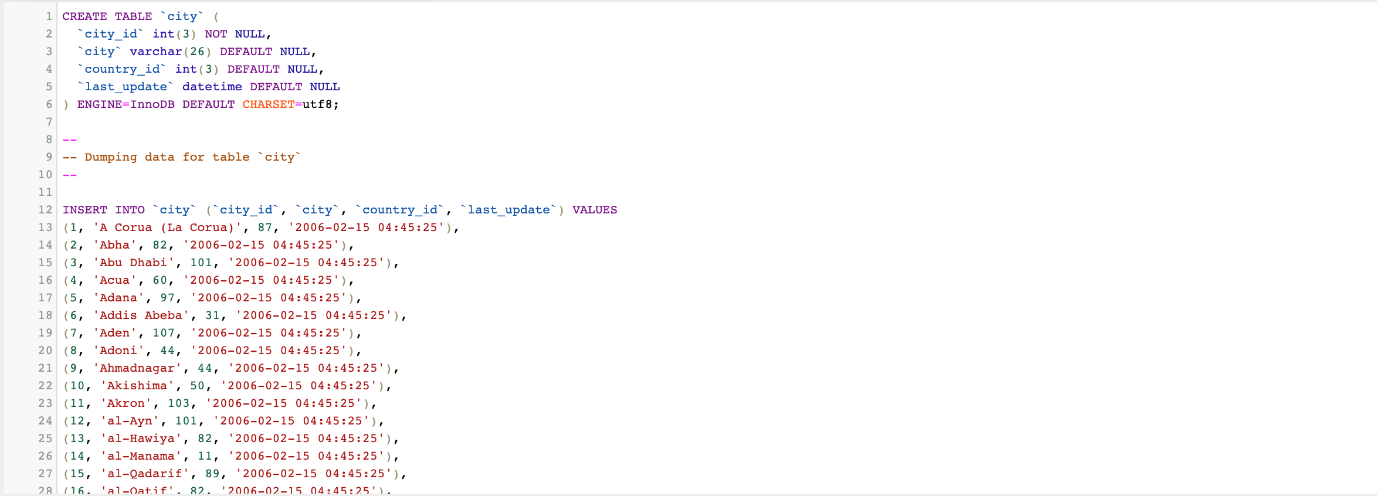
\includegraphics[width=\textwidth]{table_city_cins}
		\caption{Creation and Insertion of table "City"}	
	\end{figure}
	\begin{figure}[H]
		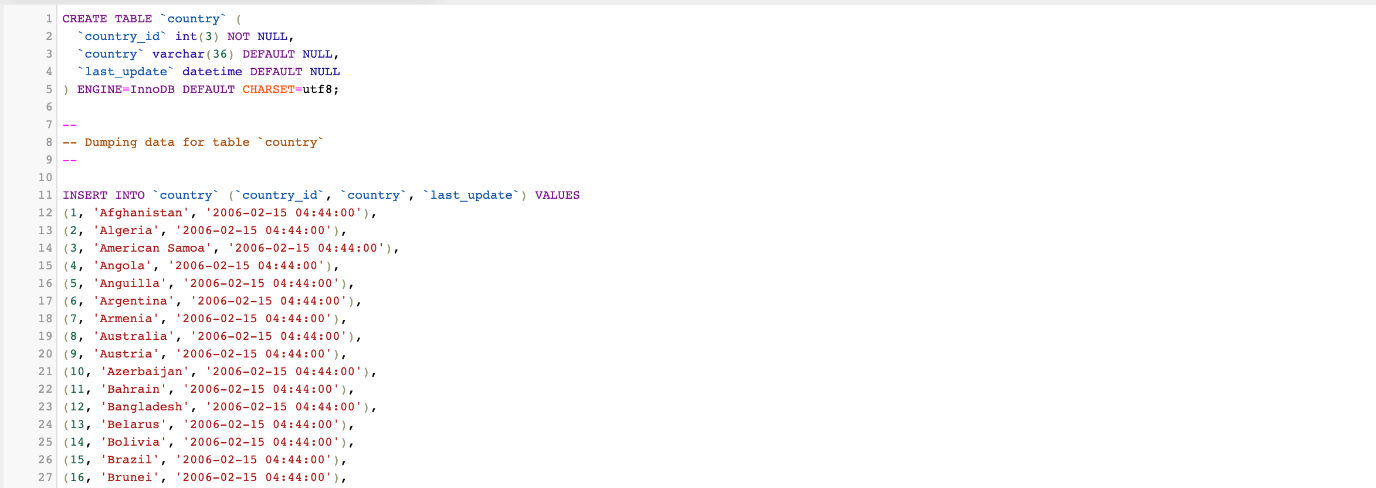
\includegraphics[width=\textwidth]{table_country_cins}
		\caption{Creation and Insertion of table "Country"}	
	\end{figure}
	\begin{figure}[H]
		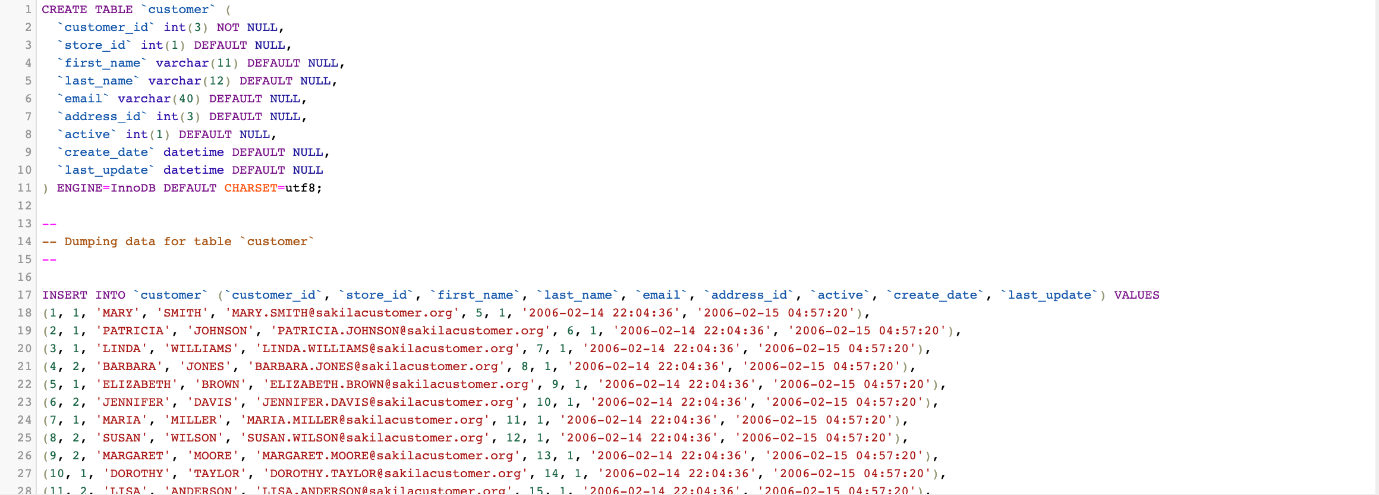
\includegraphics[width=\textwidth]{table_customer_cins}
		\caption{Creation and Insertion of table "Customer"}	
	\end{figure}
	\begin{figure}[H]
		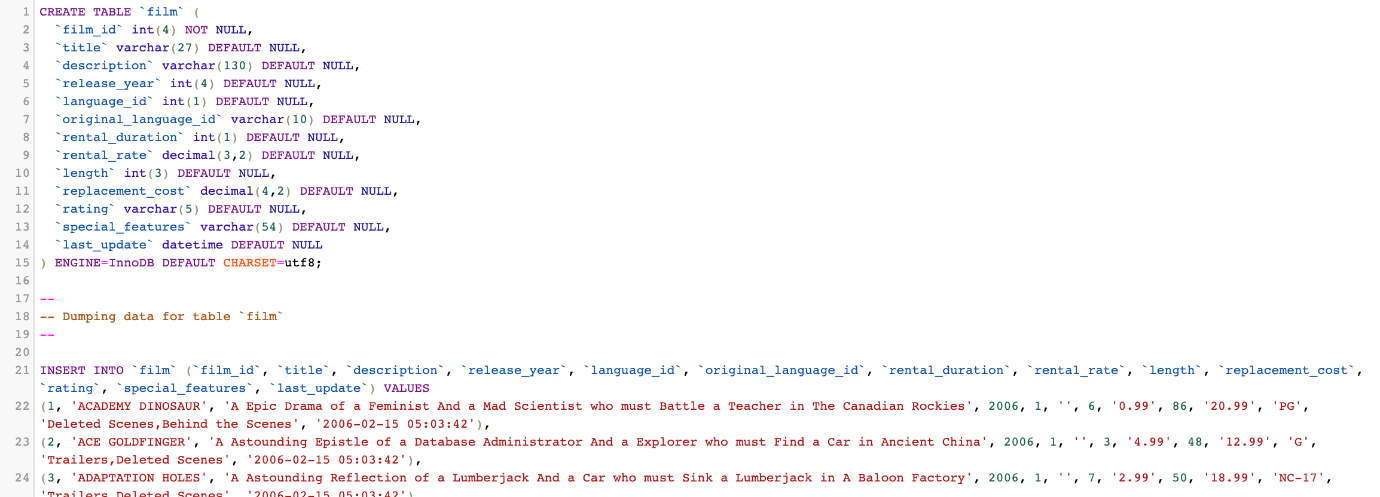
\includegraphics[width=\textwidth]{table_film_cins}
		\caption{Creation and Insertion of table "Film"}	
	\end{figure}
	\begin{figure}[H]
		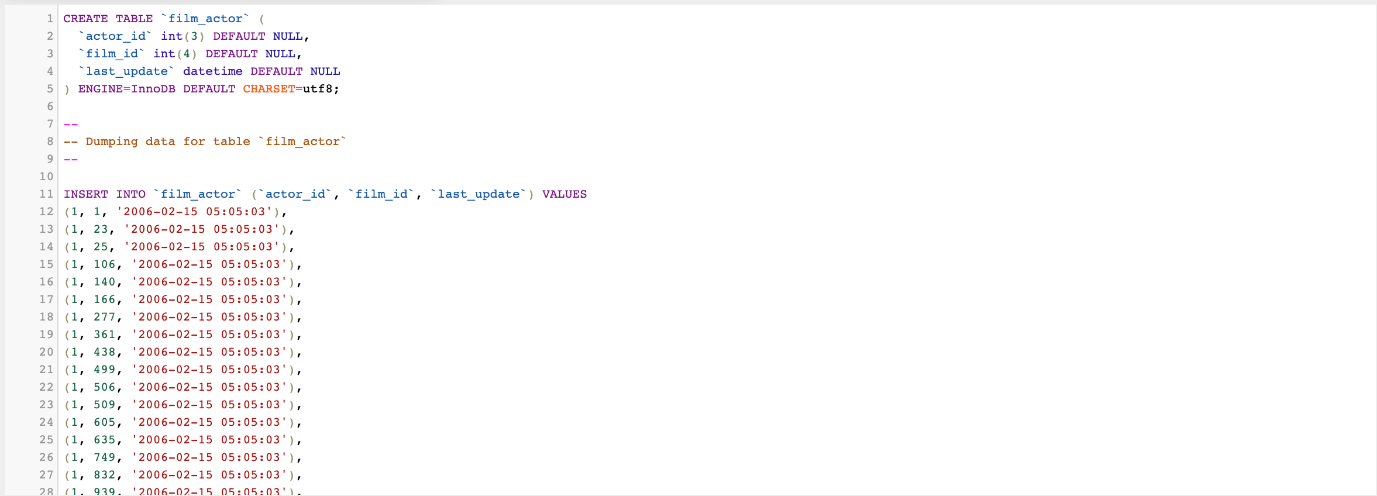
\includegraphics[width=\textwidth]{table_filmactor_cins}
		\caption{Creation and Insertion of table "Film\textunderscore Actor"}	
	\end{figure}
	\begin{figure}[H]
		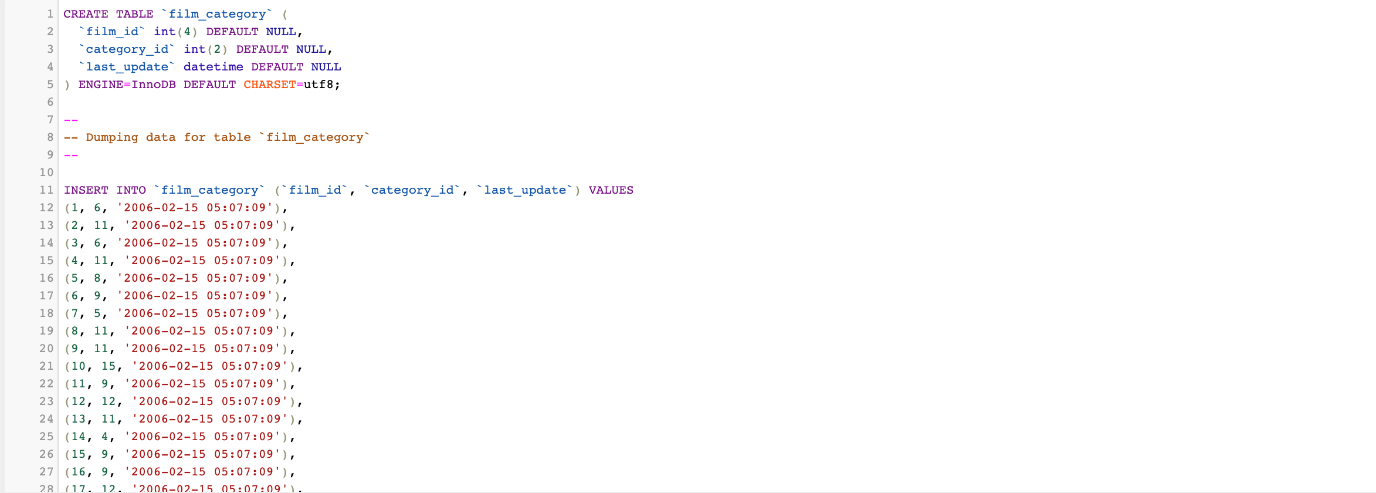
\includegraphics[width=\textwidth]{table_filmcategory_cins}
		\caption{Creation and Insertion of table "Film\textunderscore Category"}	
	\end{figure}
	\begin{figure}[H]
		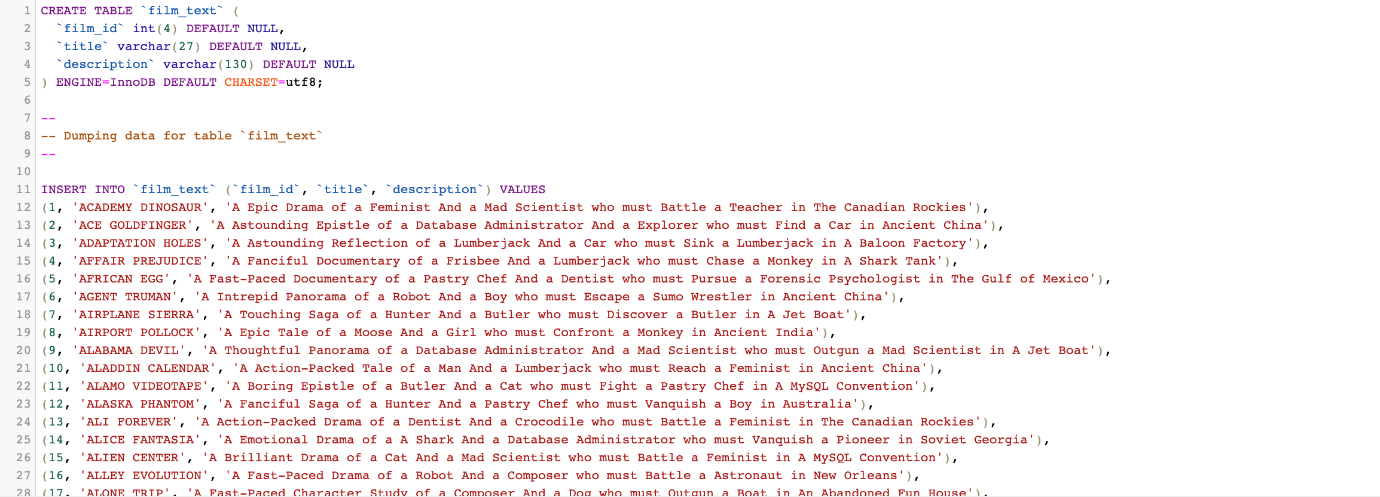
\includegraphics[width=\textwidth]{table_filmtext_cins}
		\caption{Creation and Insertion of table "Film\textunderscore Text"}	
	\end{figure}
	\begin{figure}[H]
		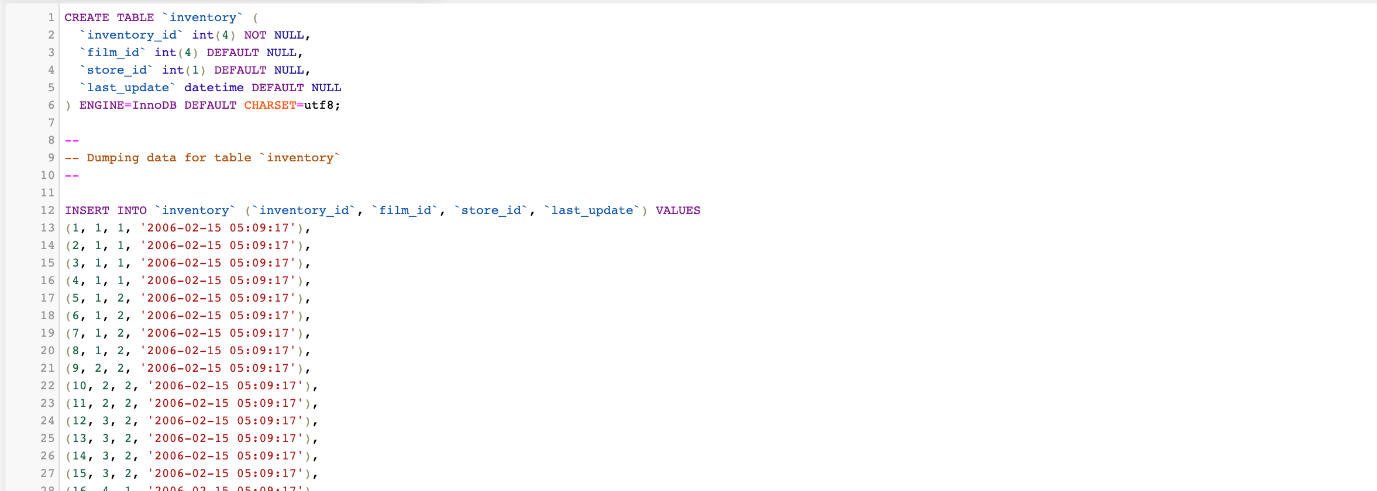
\includegraphics[width=\textwidth]{table_inventory_cins}
		\caption{Creation and Insertion of table "Inventory"}	
	\end{figure}
	\begin{figure}[H]
		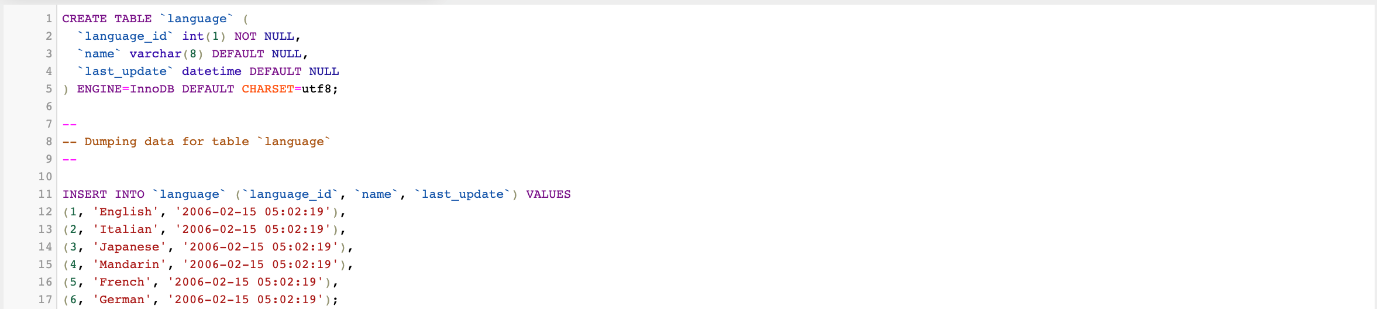
\includegraphics[width=\textwidth]{table_language_cins}
		\caption{Creation and Insertion of table "Language"}	
	\end{figure}
	\begin{figure}[H]
		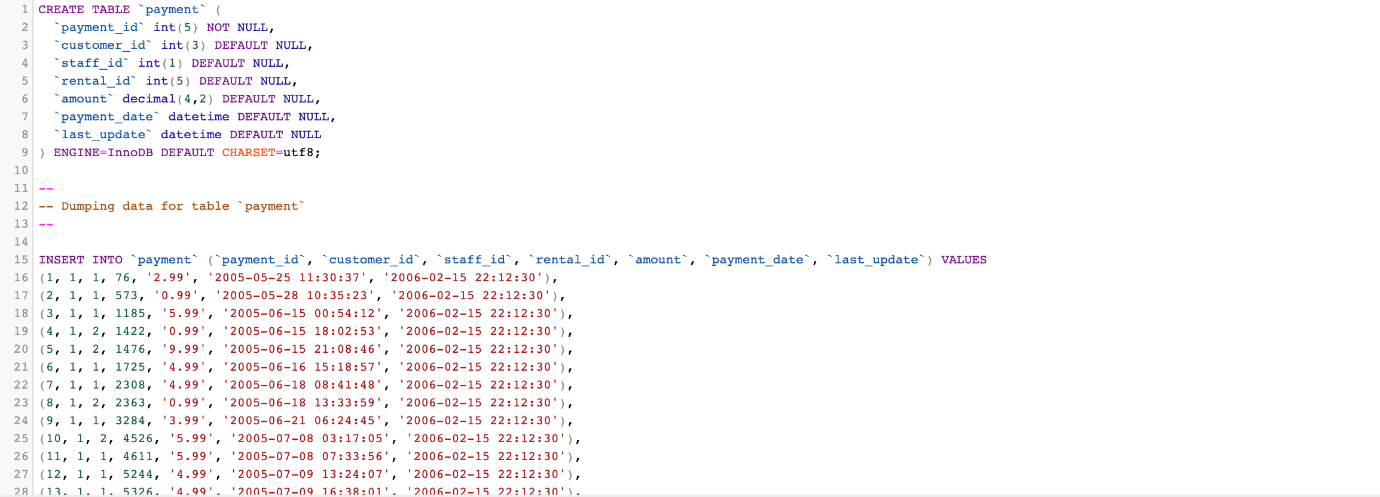
\includegraphics[width=\textwidth]{table_payment_cins}
		\caption{Creation and Insertion of table "Payment"}	
	\end{figure}
	\begin{figure}[H]
		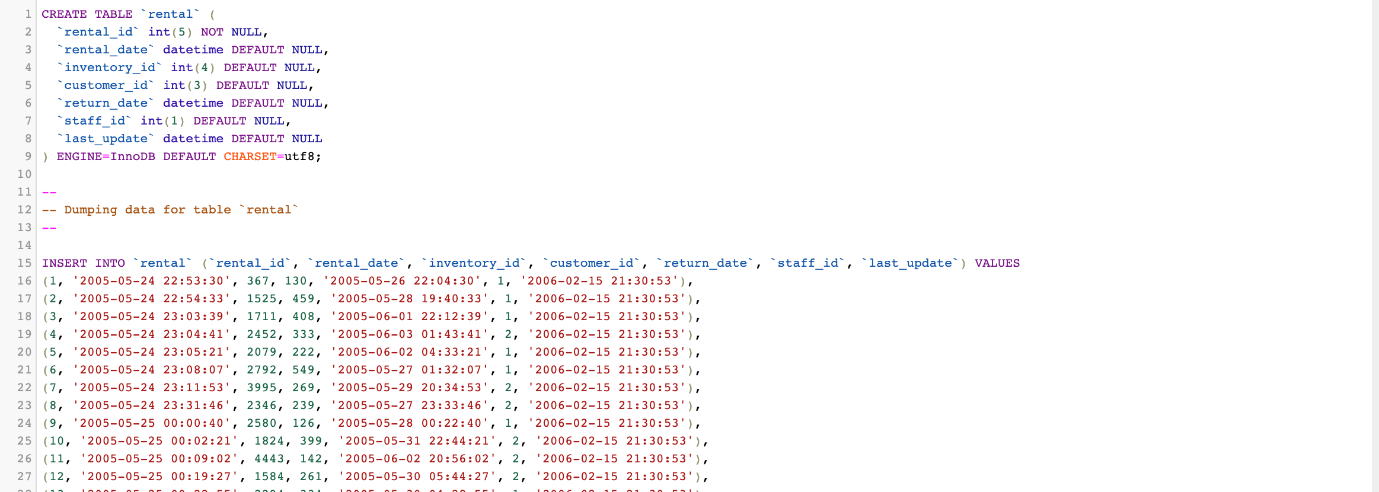
\includegraphics[width=\textwidth]{table_rental_cins}
		\caption{Creation and Insertion of table "Rental"}	
	\end{figure}
	\begin{figure}[H]
		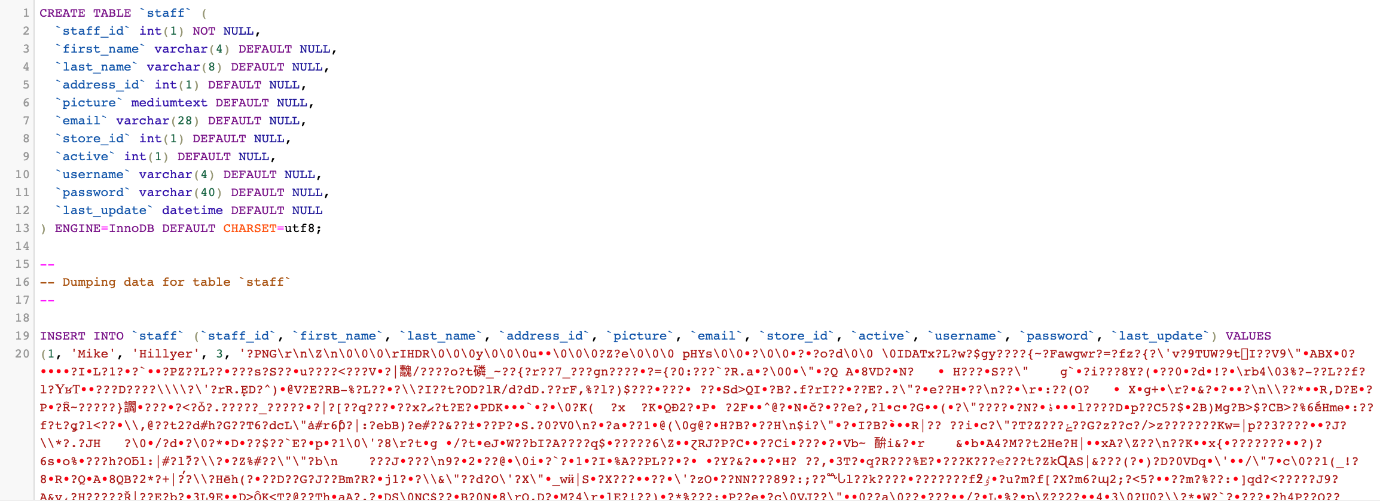
\includegraphics[width=\textwidth]{table_staff_cins}
		\caption{Creation and Insertion of table "Staff"}	
	\end{figure}
	\begin{figure}[H]
		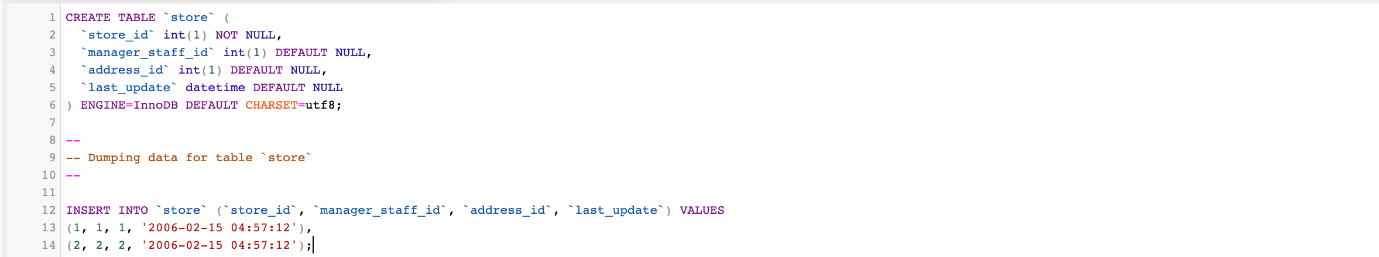
\includegraphics[width=\textwidth]{table_store_cins}
		\caption{Creation and Insertion of table "Store"}	
	\end{figure}

\section{Table Constraints (Foreign Keys)}
	\begin{figure}[H]
		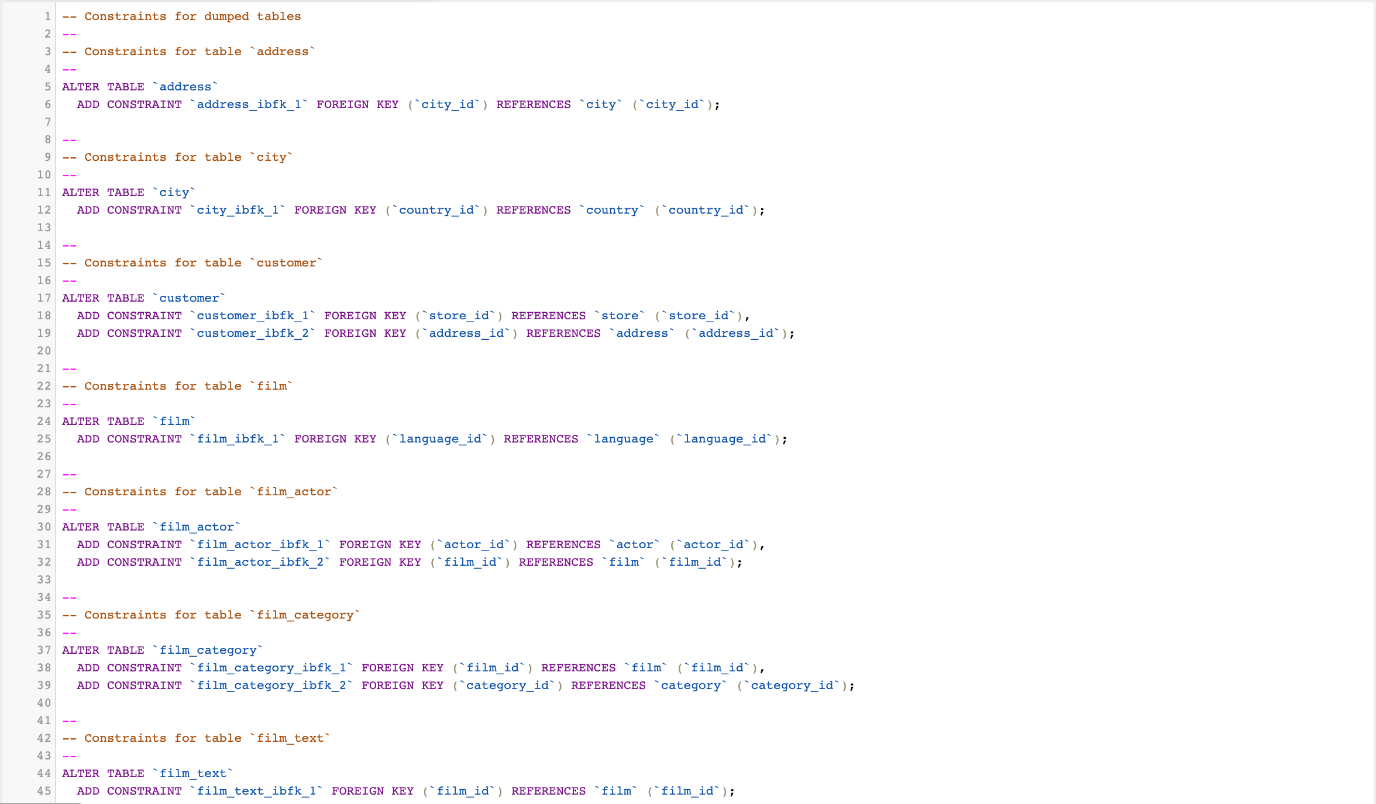
\includegraphics[width=\textwidth]{tableconstraints1}
		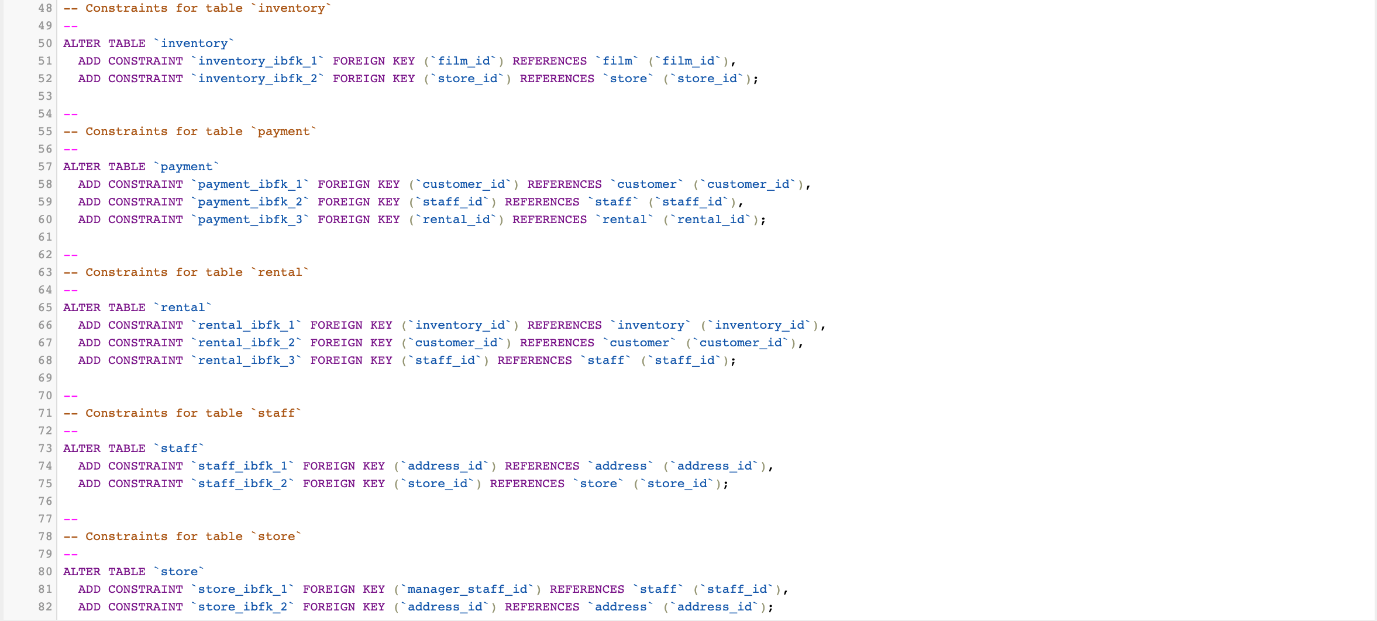
\includegraphics[width=\textwidth]{tableconstraints2}
	\end{figure}

\section{Table Indexes (Primary/Foreign Keys)}
	\begin{figure}[H]
		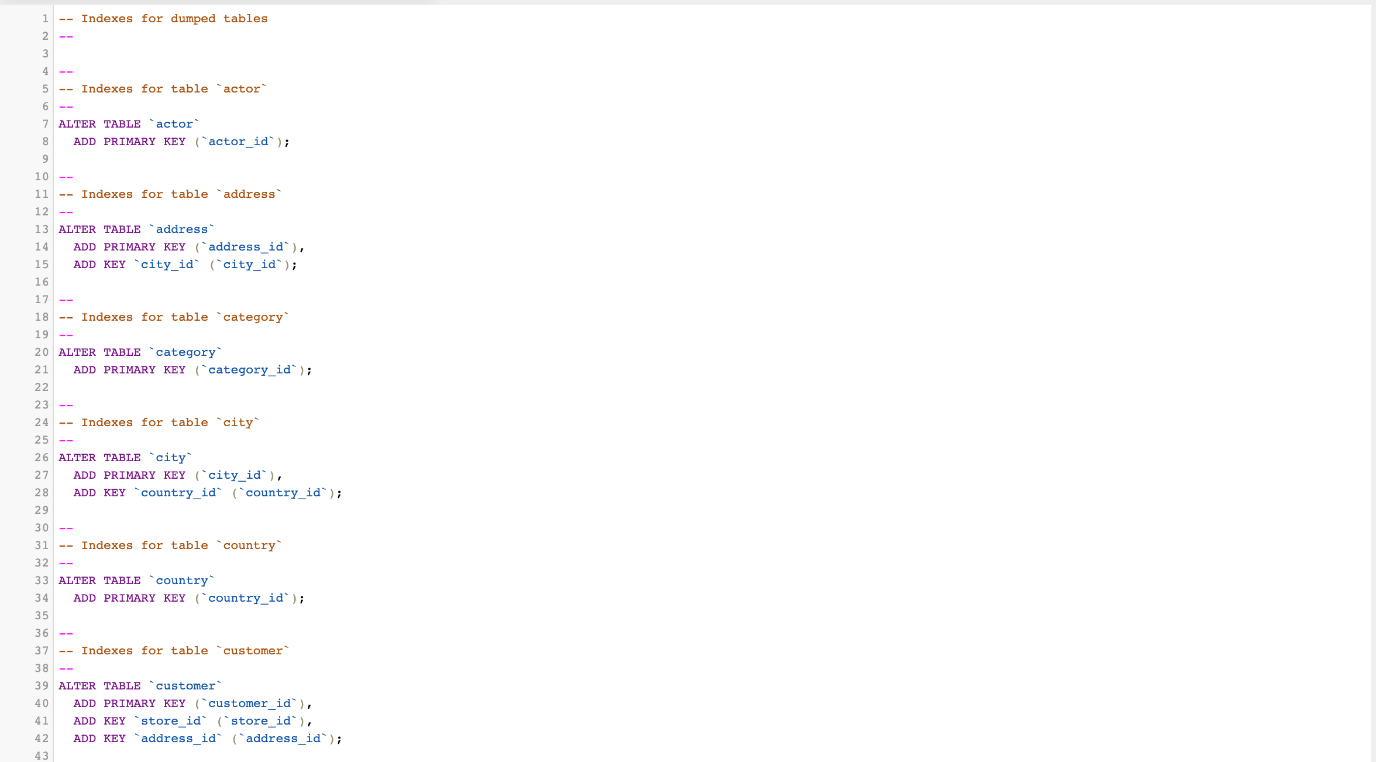
\includegraphics[width=\textwidth]{tableindexkeys1}
		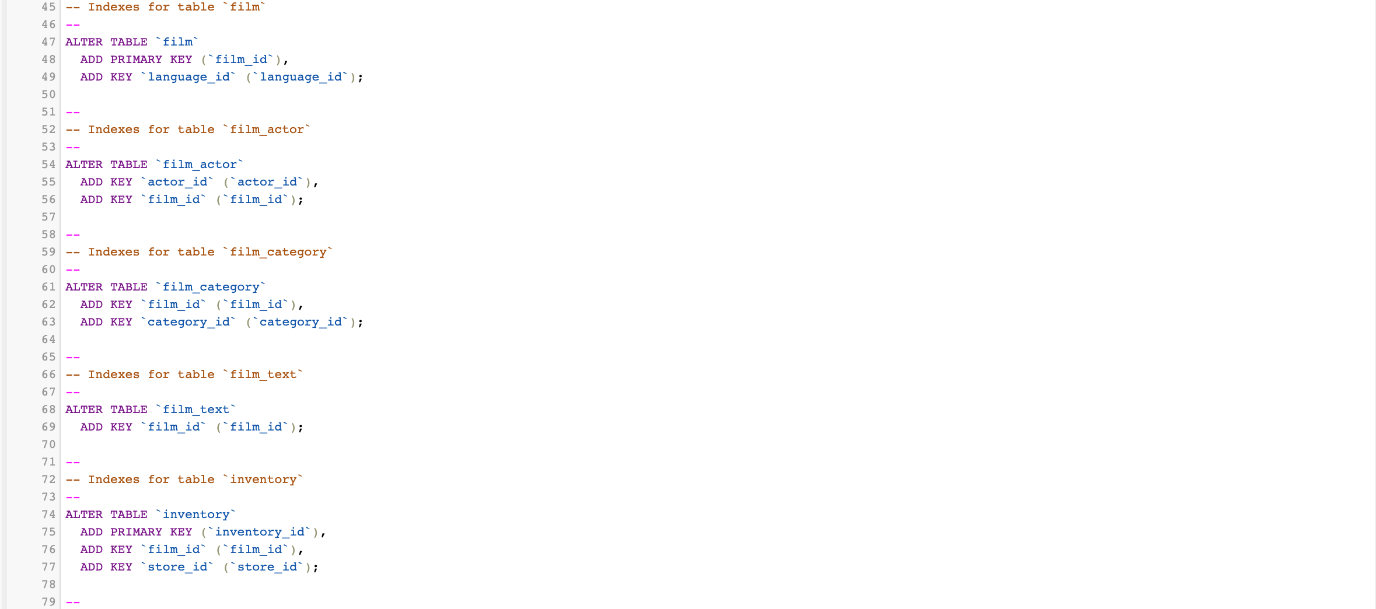
\includegraphics[width=\textwidth]{tableindexkeys2}
		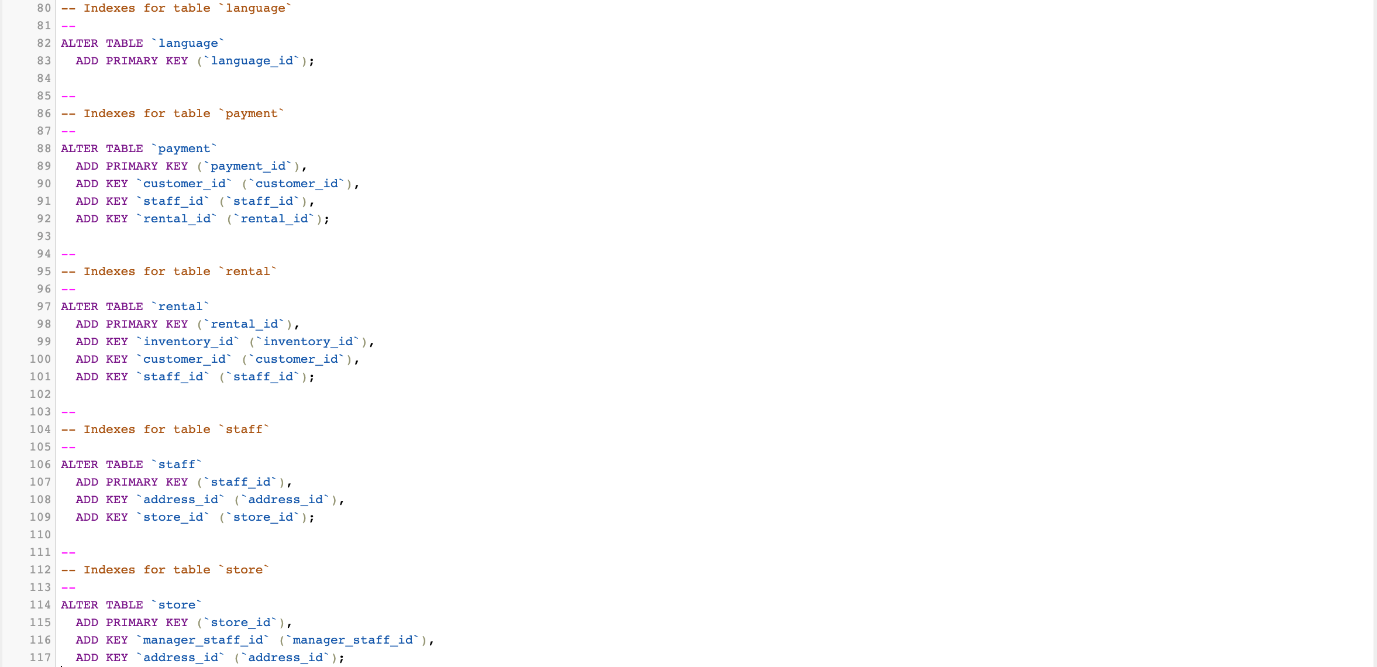
\includegraphics[width=\textwidth]{tableindexkeys3}
	\end{figure}	

\section{Table Structures}
	\begin{figure}[H]
		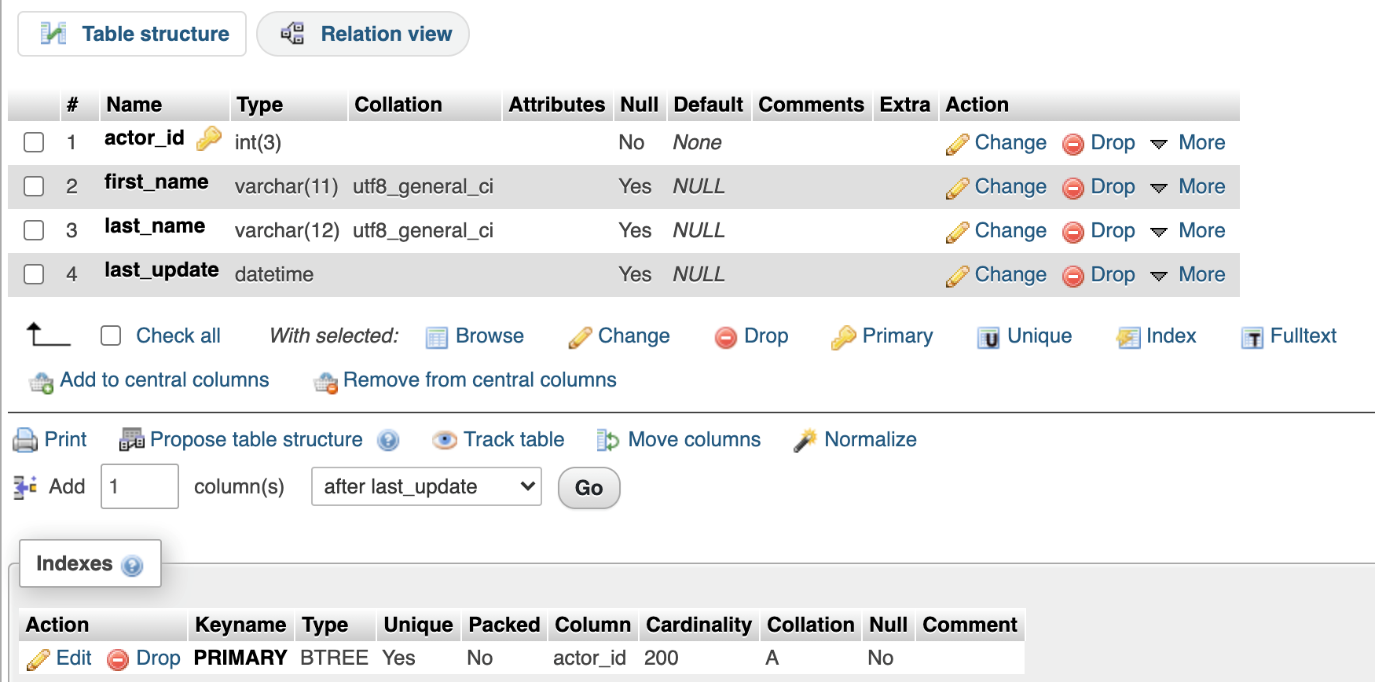
\includegraphics[width=\textwidth]{table_actor_struct}
		\caption{Structure of table "Actor"}	
	\end{figure}
	\begin{figure}[H]
		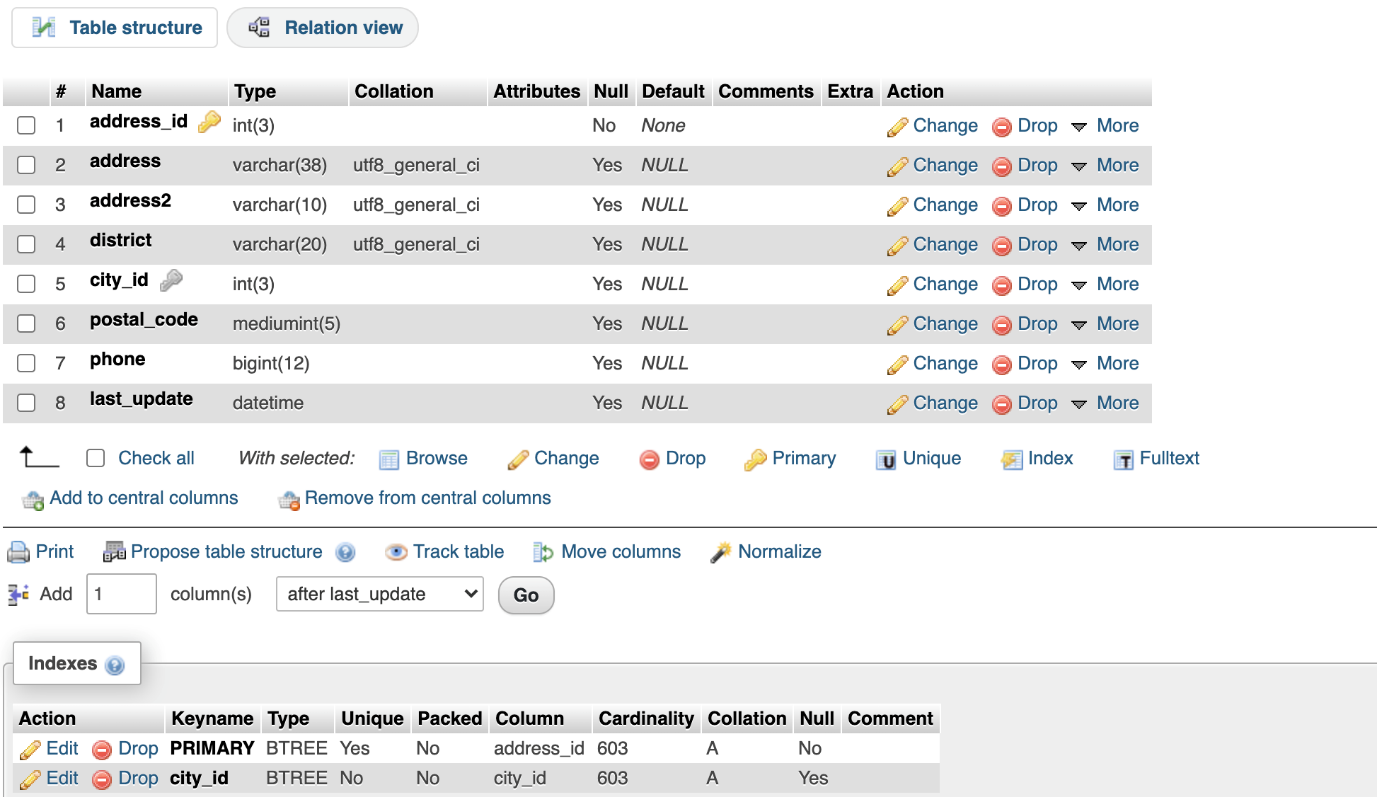
\includegraphics[width=\textwidth]{table_address_struct}
		\caption{Structure of table "Address"}	
	\end{figure}
	\begin{figure}[H]
		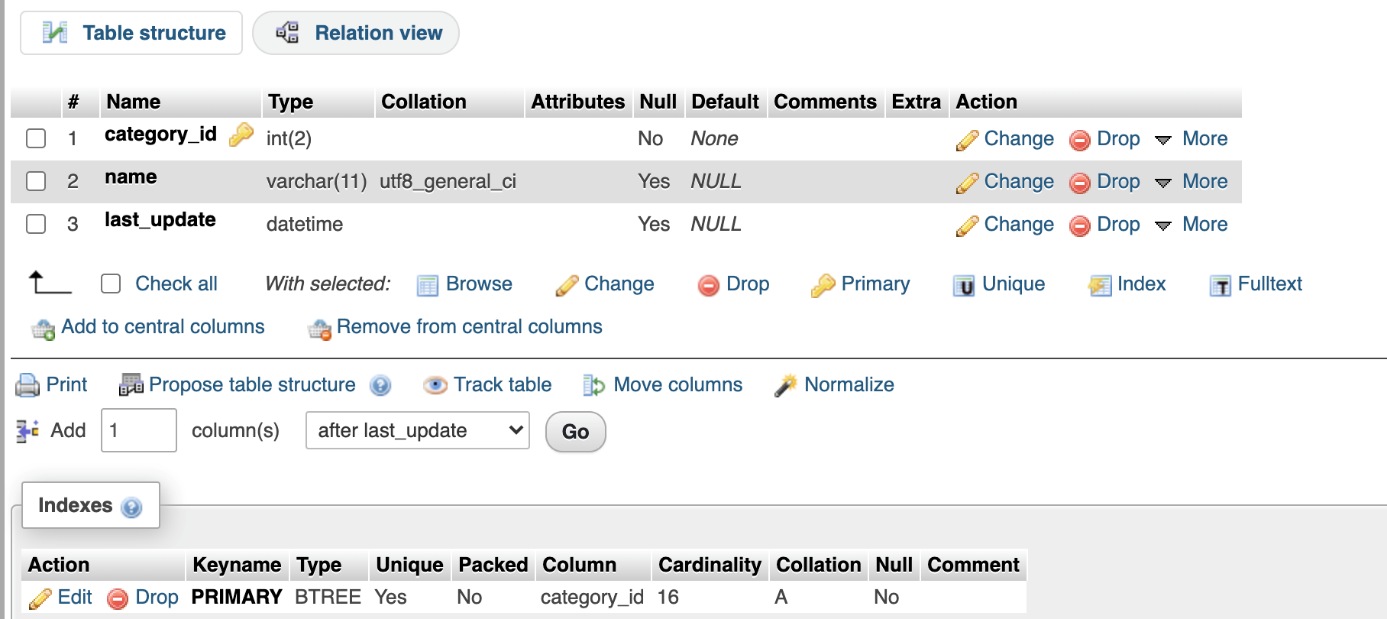
\includegraphics[width=\textwidth]{table_category_struct}
		\caption{Structure of table "Category"}	
	\end{figure}
	\begin{figure}[H]
		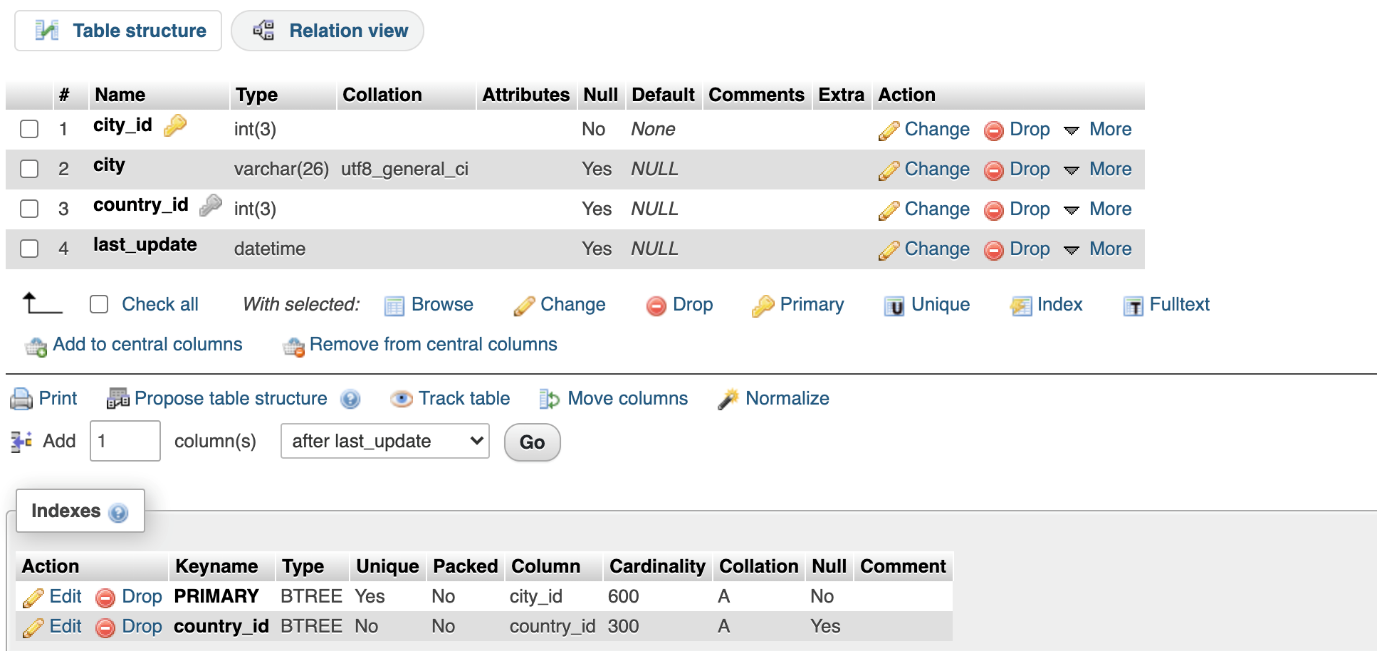
\includegraphics[width=\textwidth]{table_city_struct}
		\caption{Structure of table "City"}	
	\end{figure}
	\begin{figure}[H]
		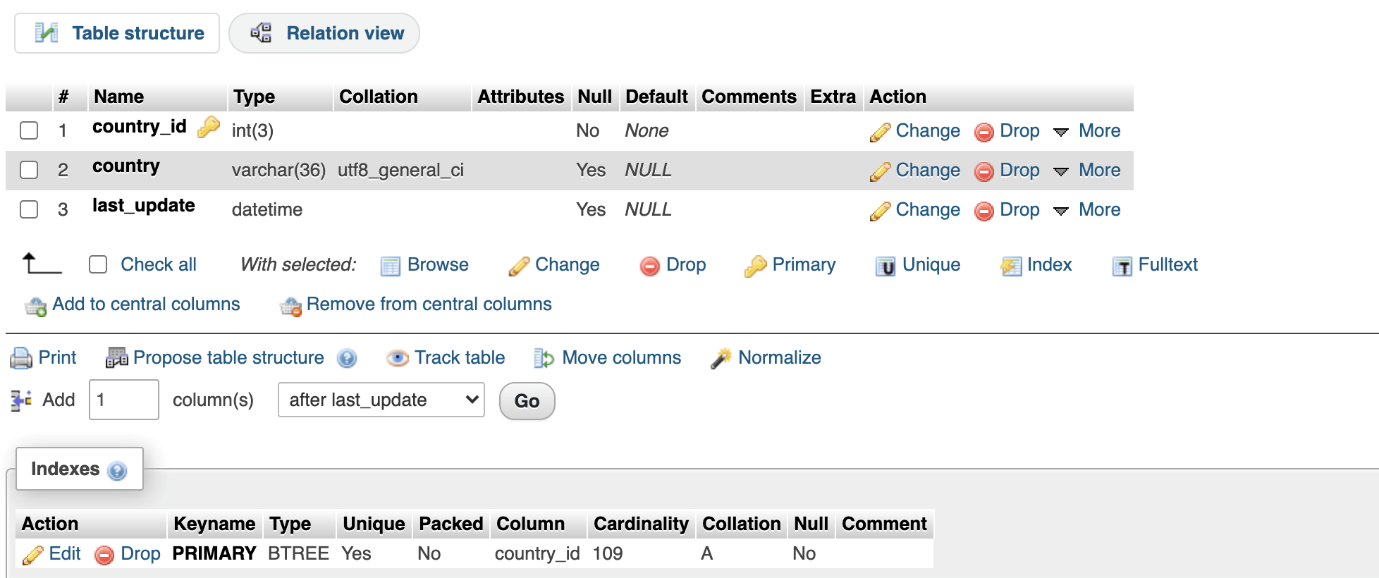
\includegraphics[width=\textwidth]{table_country_struct}
		\caption{Structure of table "Country"}	
	\end{figure}
	\begin{figure}[H]
		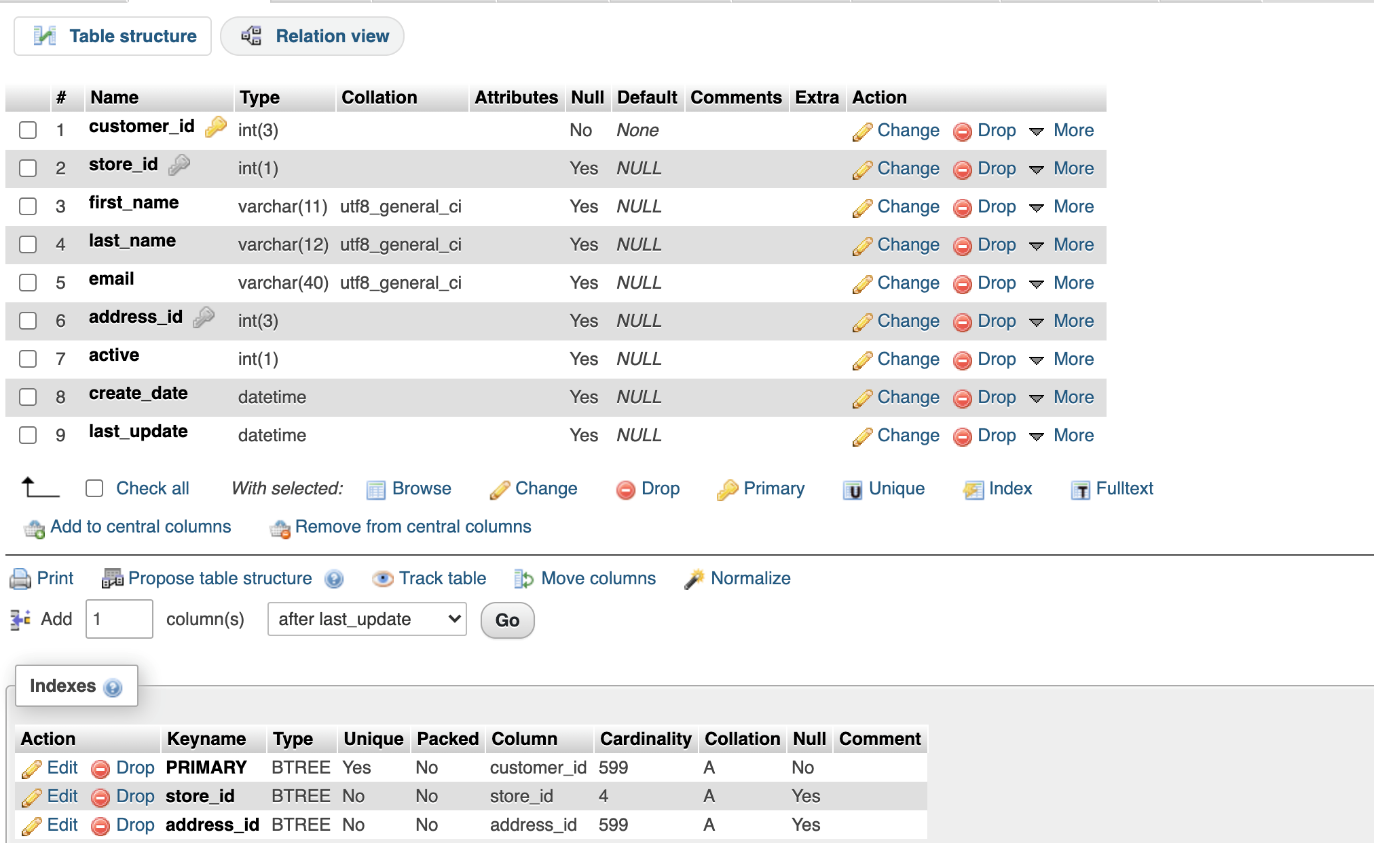
\includegraphics[width=\textwidth]{table_customer_struct}
		\caption{Structure of table "Customer"}	
	\end{figure}
	\begin{figure}[H]
		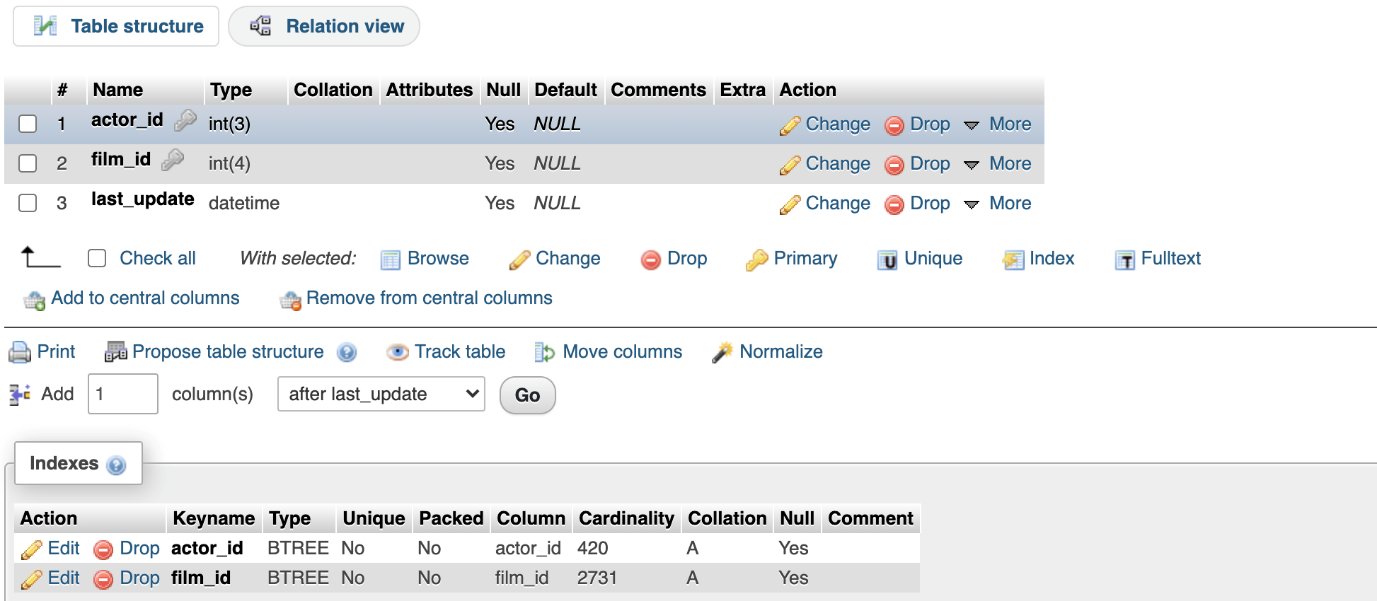
\includegraphics[width=\textwidth]{table_filmactor_struct}
		\caption{Structure of table "Film\textunderscore Actor"}	
	\end{figure}
	\begin{figure}[H]
		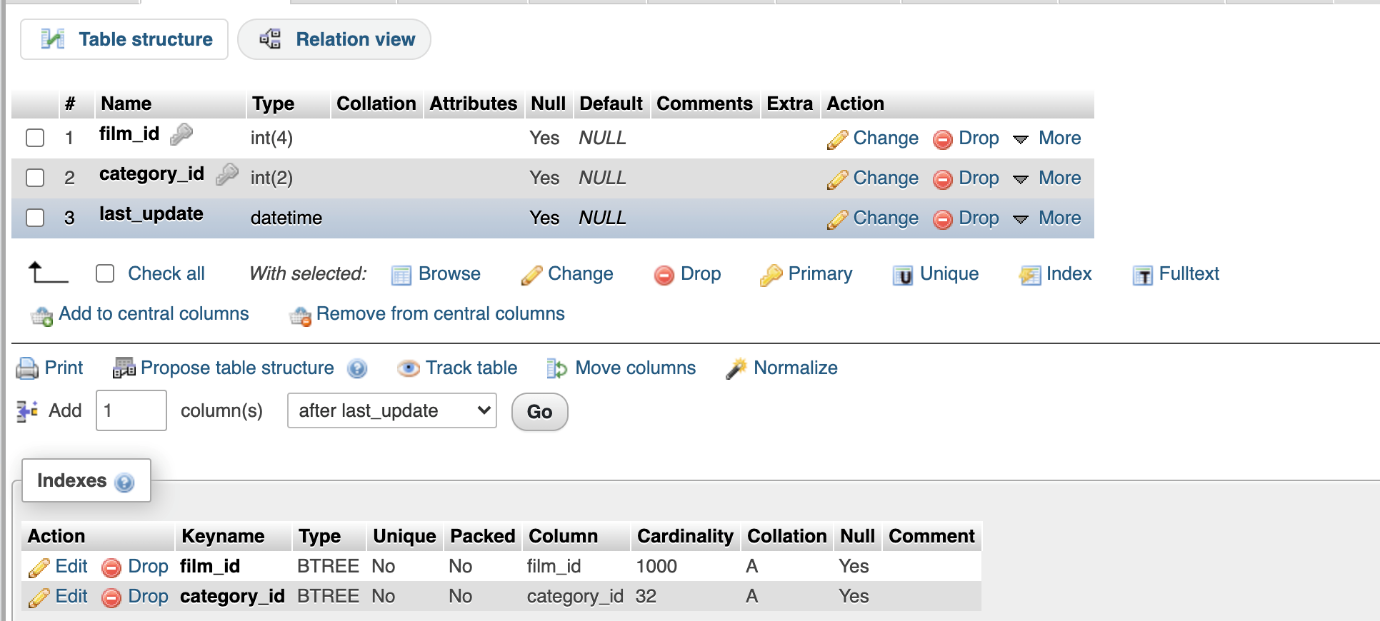
\includegraphics[width=\textwidth]{table_filmcategory_struct}
		\caption{Structure of table "Film\textunderscore Category"}	
	\end{figure}
	\begin{figure}[H]
		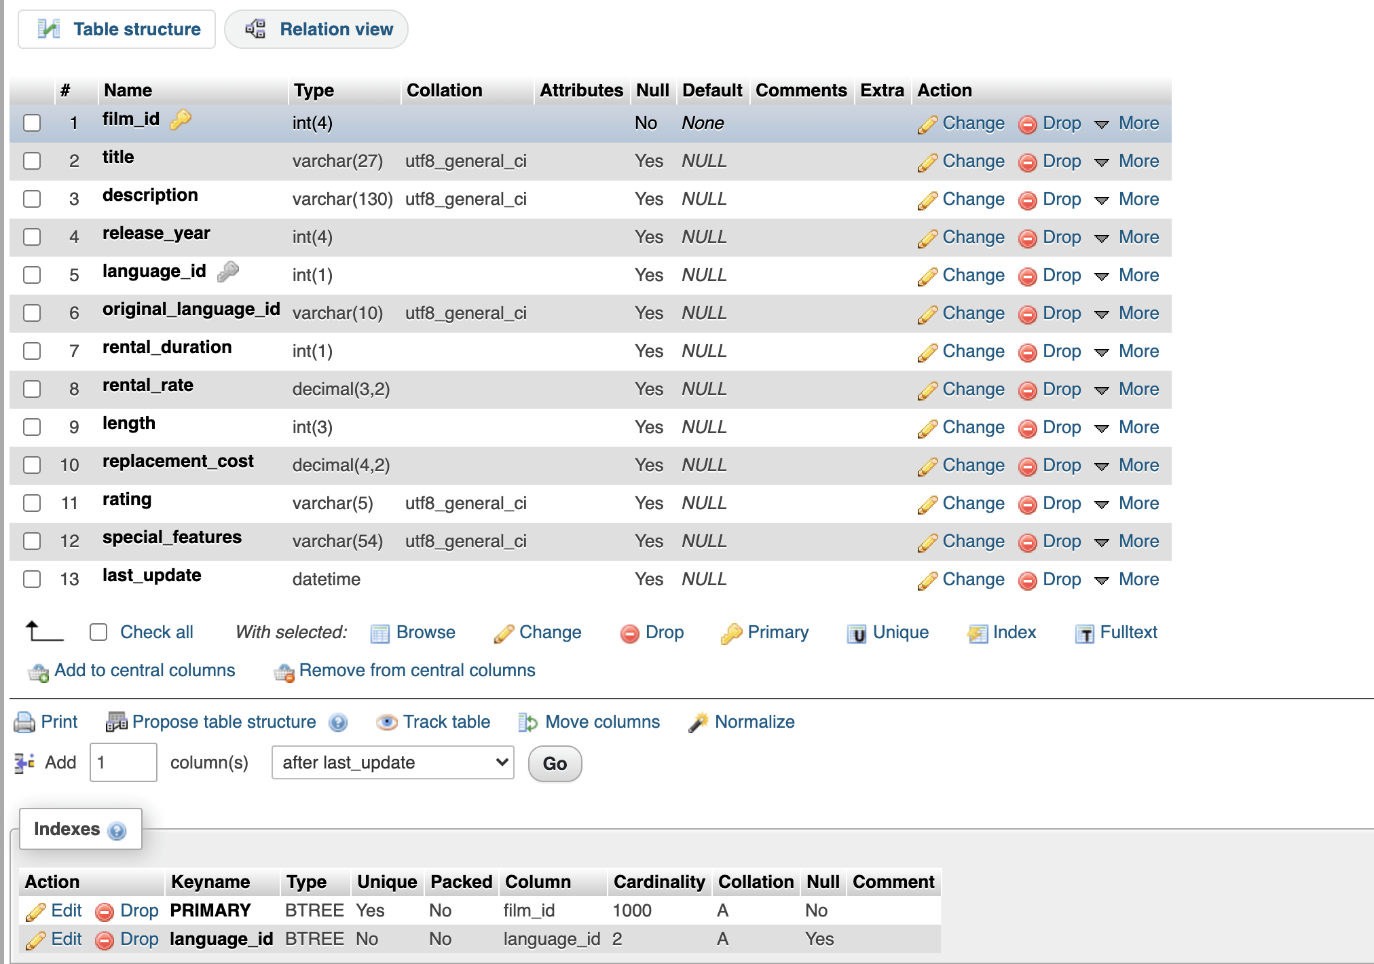
\includegraphics[width=\textwidth]{table_film_struct}
		\caption{Structure of table "Film"}	
	\end{figure}
	\begin{figure}[H]
		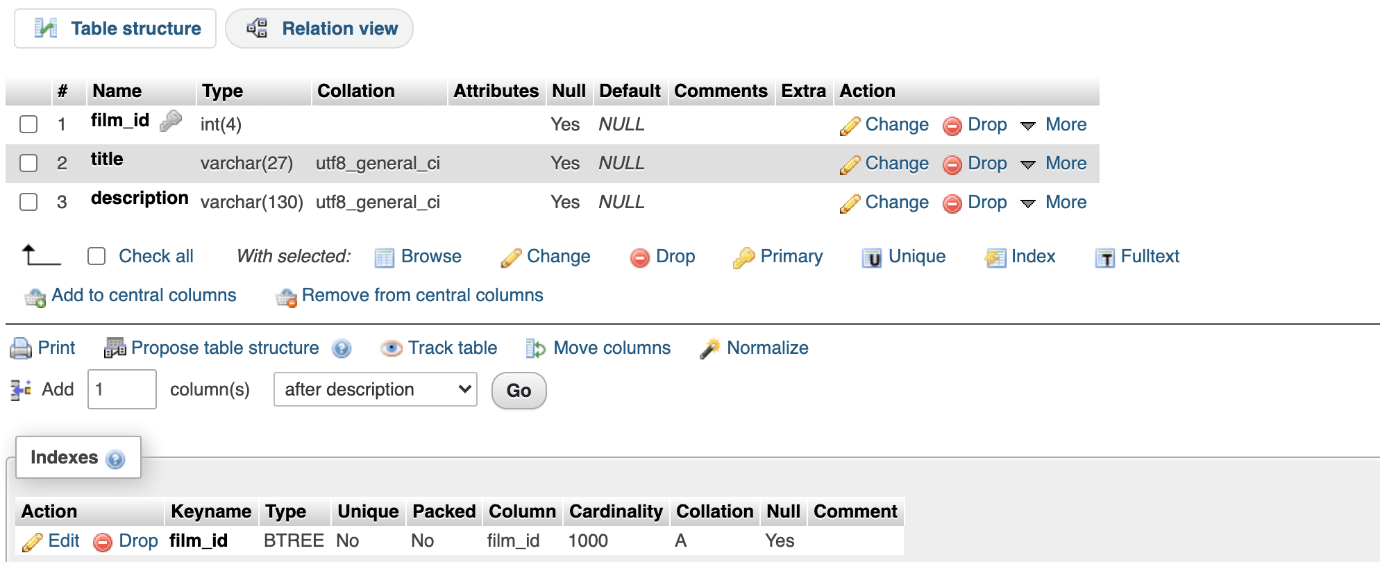
\includegraphics[width=\textwidth]{table_filmtext_struct}
		\caption{Structure of table "Film\textunderscore Text"}	
	\end{figure}
	\begin{figure}[H]
		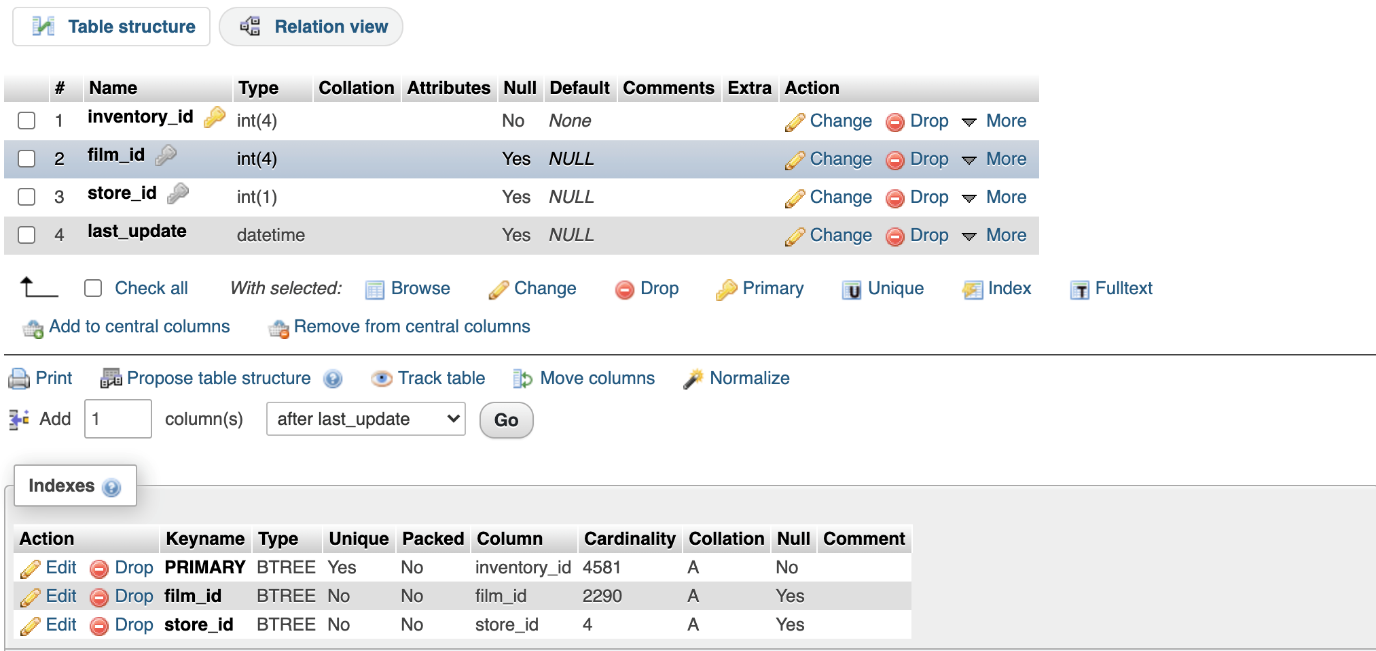
\includegraphics[width=\textwidth]{table_inventory_struct}
		\caption{Structure of table "Inventory"}	
	\end{figure}
	\begin{figure}[H]
		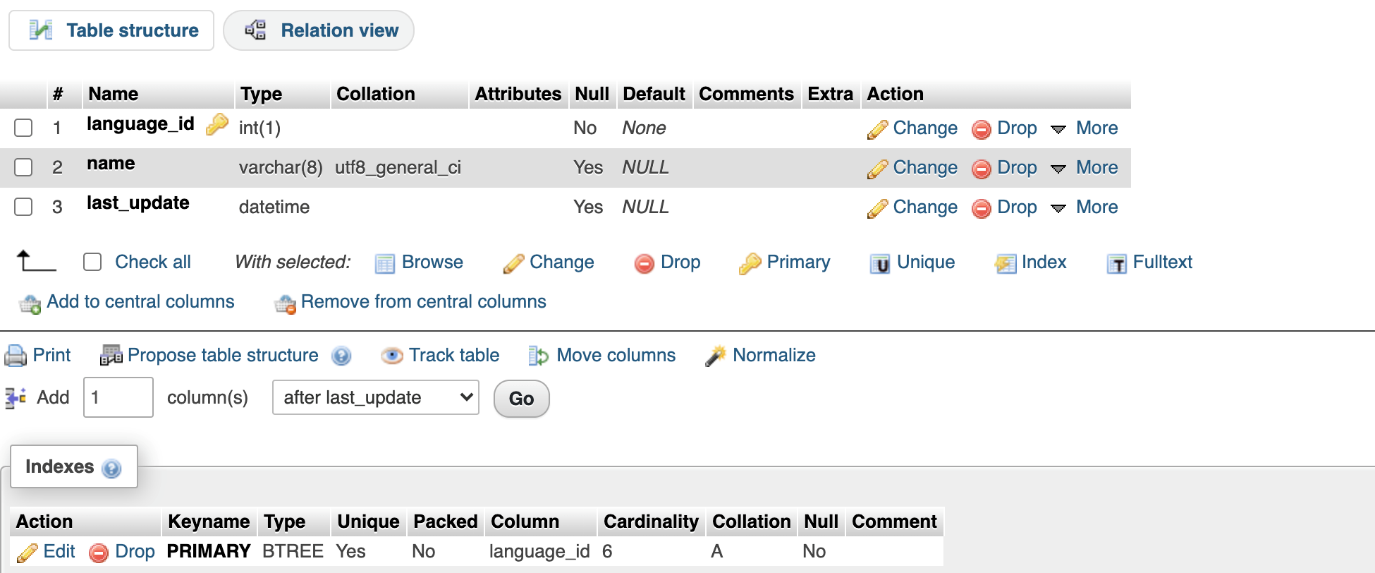
\includegraphics[width=\textwidth]{table_language_struct}
		\caption{Structure of table "Language"}	
	\end{figure}
	\begin{figure}[H]
		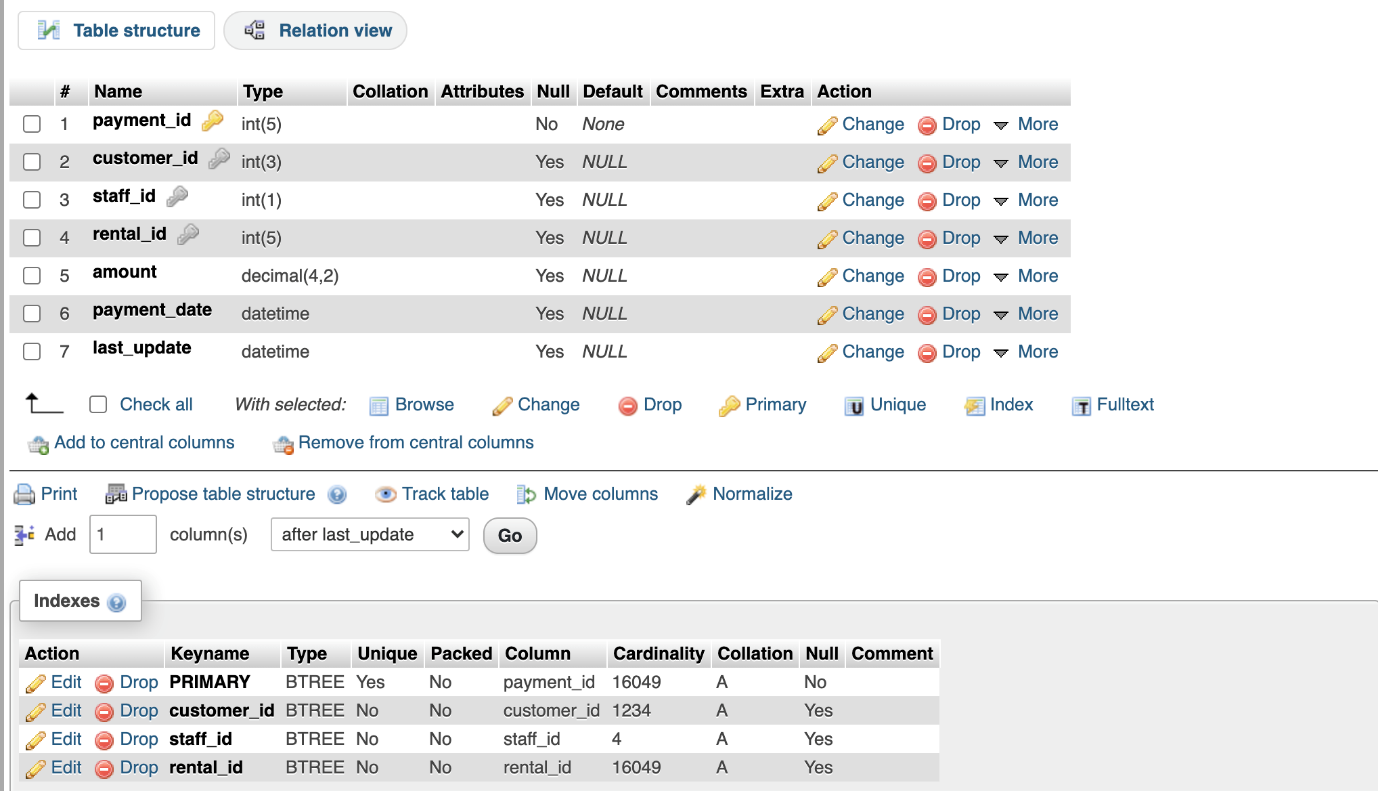
\includegraphics[width=\textwidth]{table_payment_struct}
		\caption{Structure of table "Payment"}	
	\end{figure}
	\begin{figure}[H]
		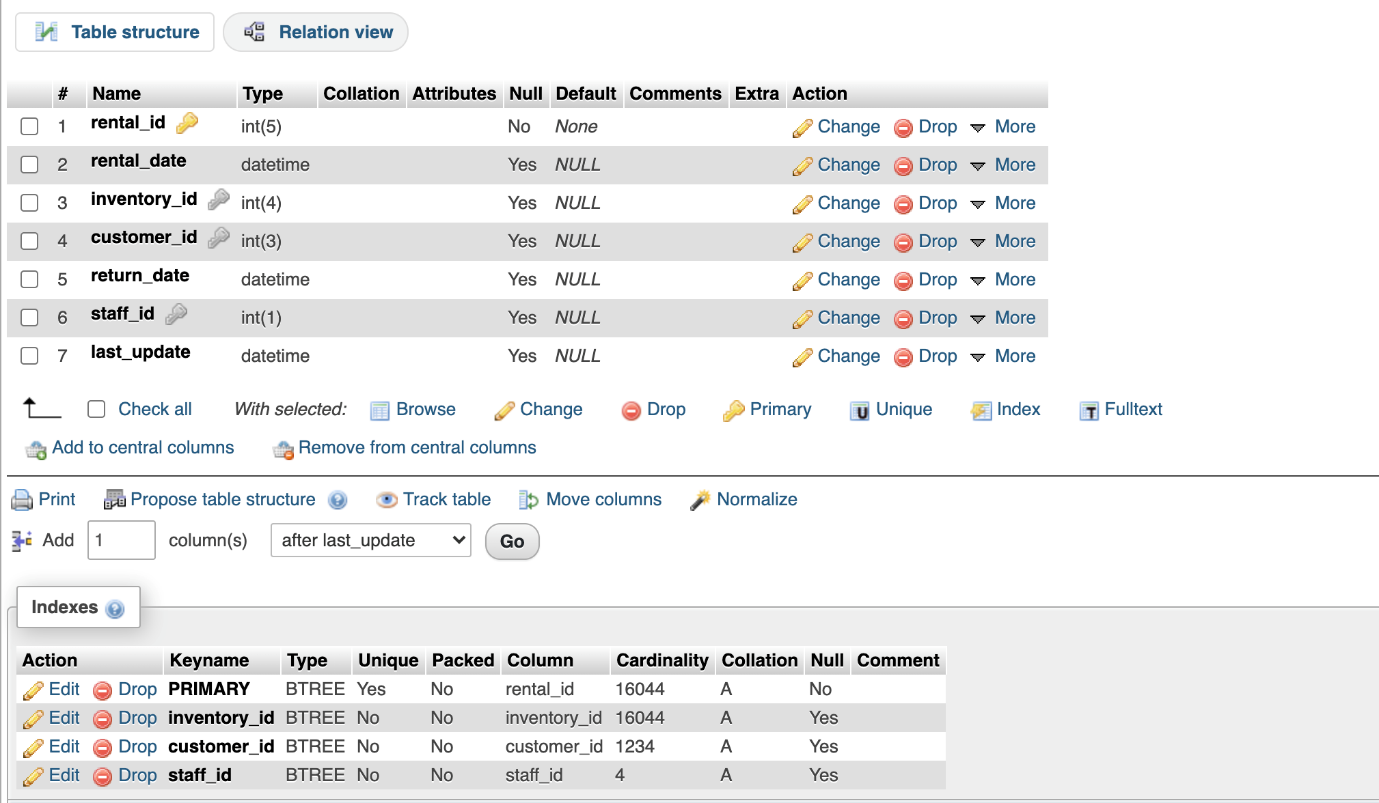
\includegraphics[width=\textwidth]{table_rental_struct}
		\caption{Structure of table "Rental"}	
	\end{figure}
	\begin{figure}[H]
		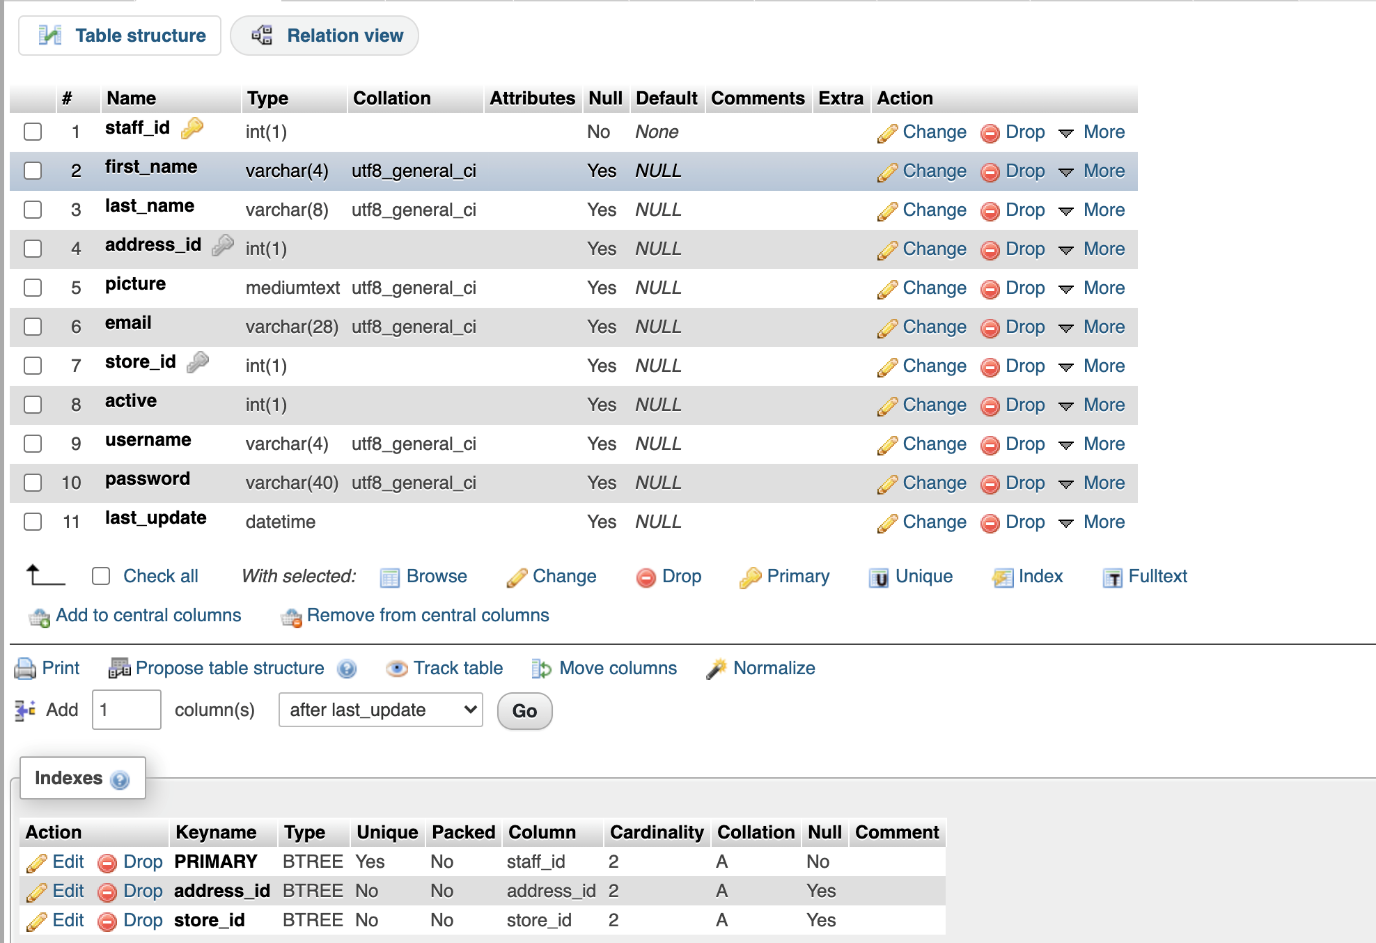
\includegraphics[width=\textwidth]{table_staff_struct}
		\caption{Structure of table "Staff"}	
	\end{figure}
	\begin{figure}[H]
		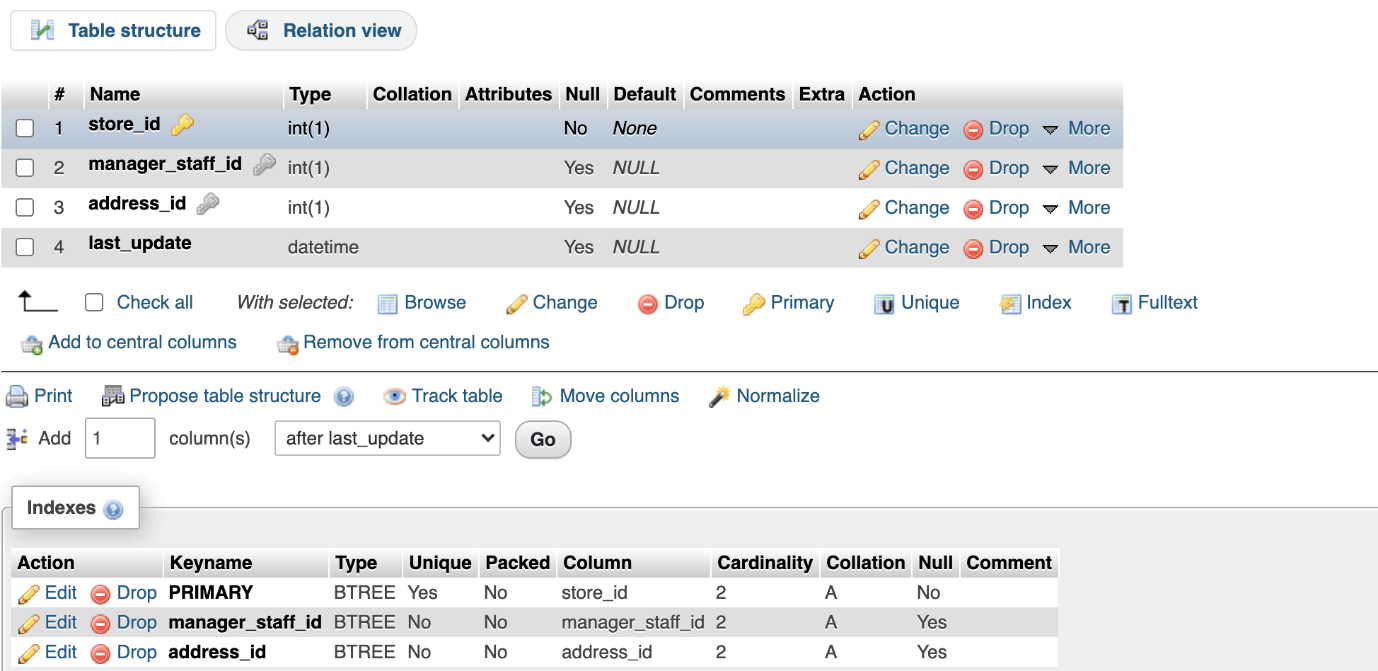
\includegraphics[width=\textwidth]{table_store_struct}
		\caption{Structure of table "Store"}	
	\end{figure}

\section{Final Results of Data Insertion \& Selection}
	\begin{figure}[H]
		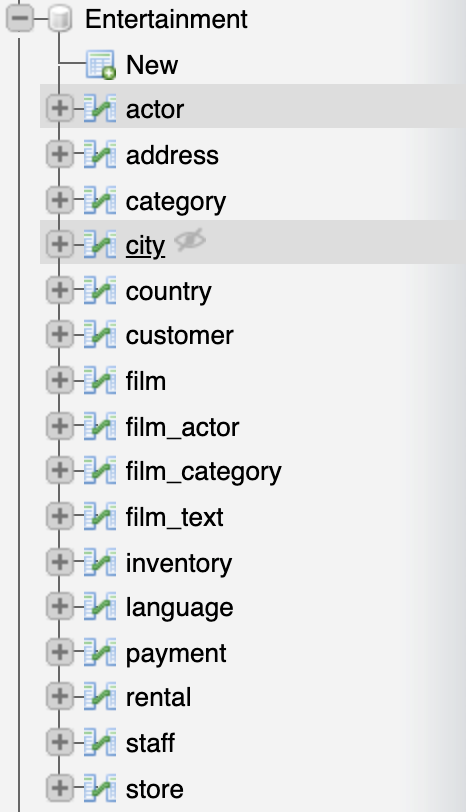
\includegraphics[width=\textwidth]{data_insertion_selection}
	\end{figure}	

\section{Overview on Tables of Database "Entertainment"}
	\begin{figure}[H]
		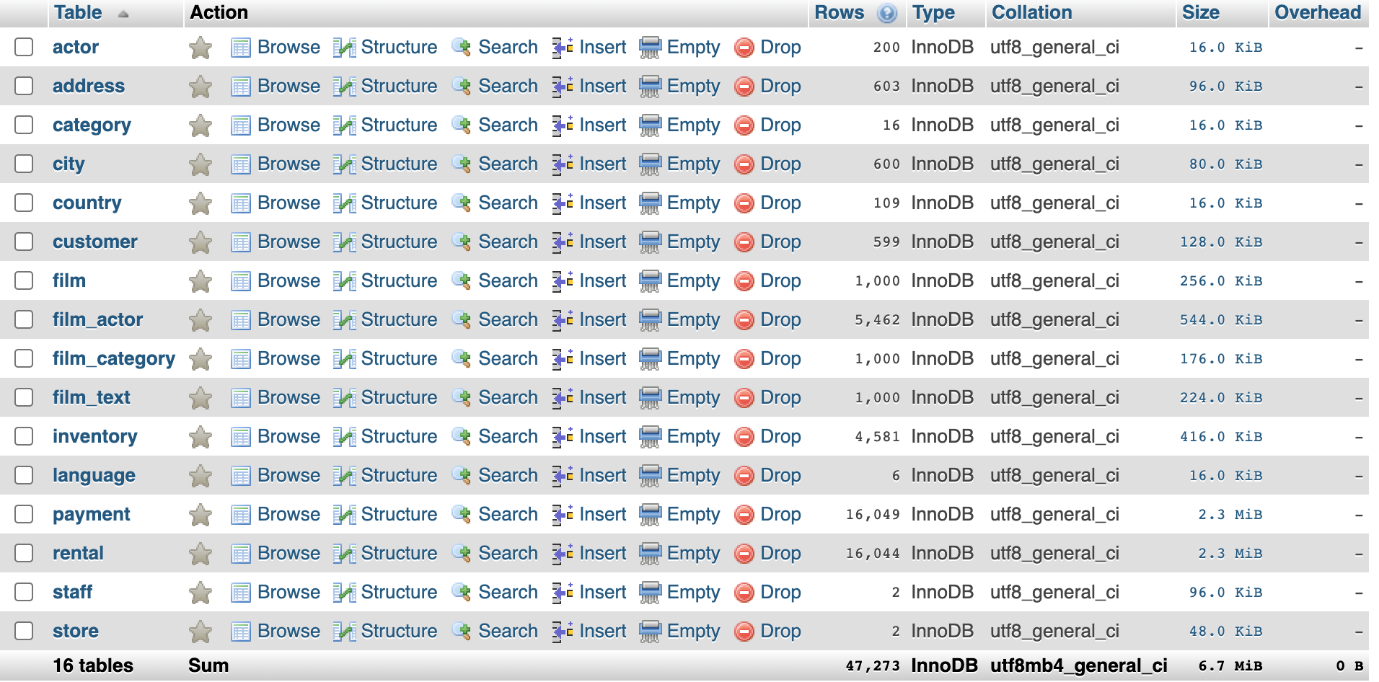
\includegraphics[width=\textwidth]{table_overview}
		\caption{Summary of tables within the database.}
	\end{figure}	
	
	\subsection{Table Contents}
		\begin{figure}[H]
			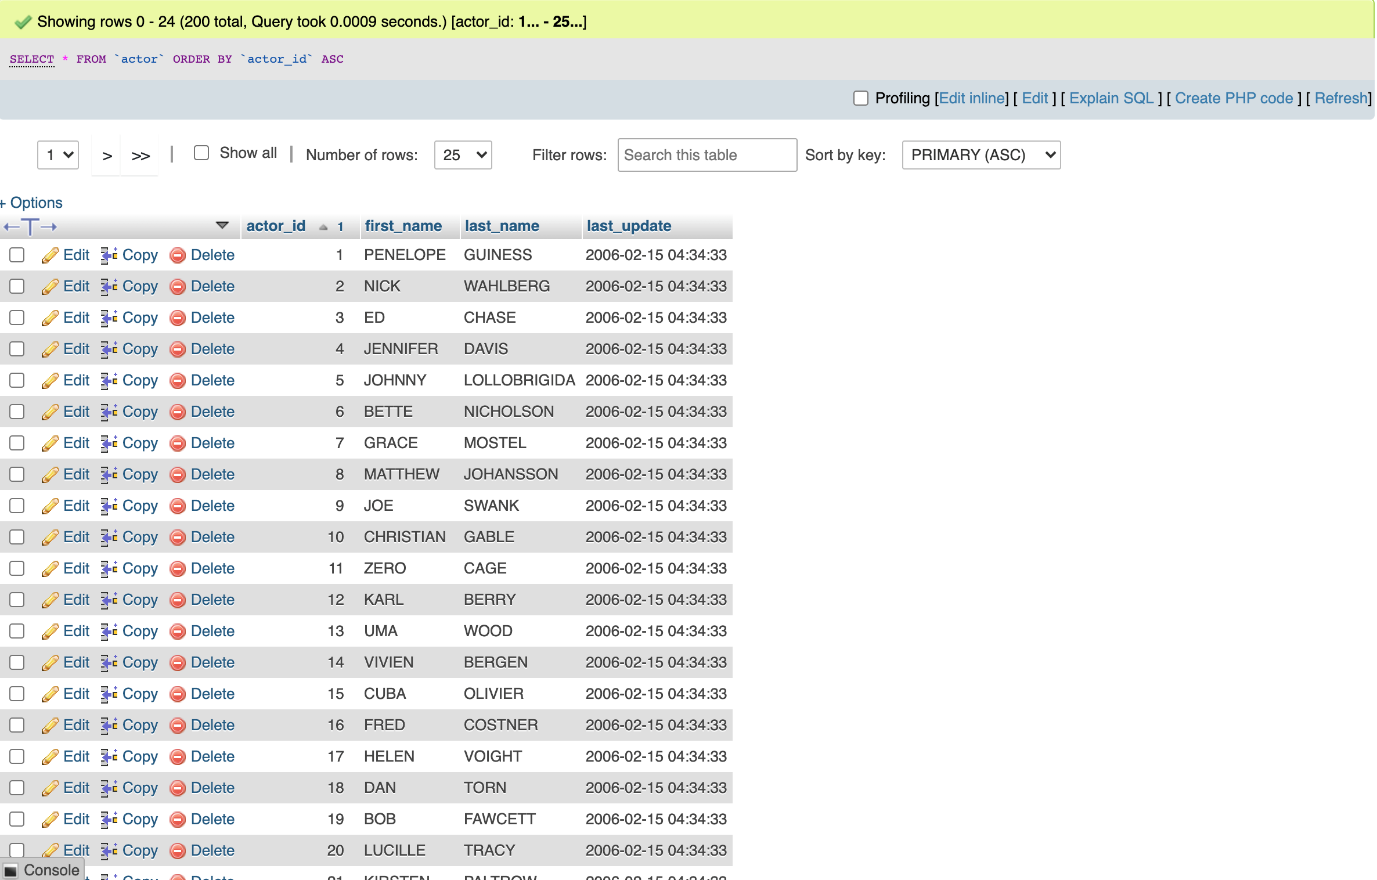
\includegraphics[width=\textwidth]{actor_content}
			\caption{Sample content of the table "Actor".}
		\end{figure}
		\begin{figure}[H]
			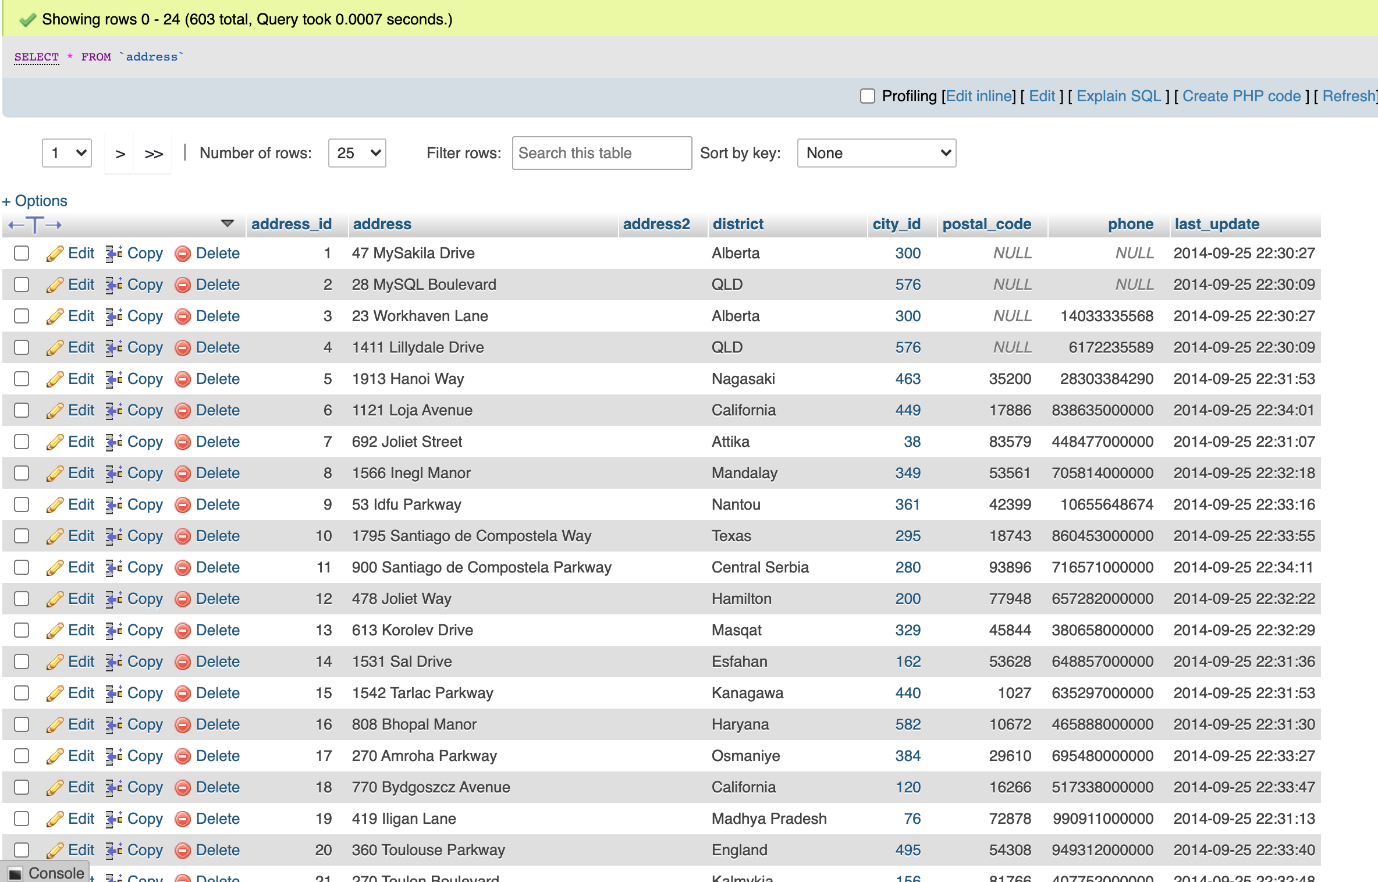
\includegraphics[width=\textwidth]{address_content}
			\caption{Sample content of the table "Address".}
		\end{figure}
		\begin{figure}[H]
			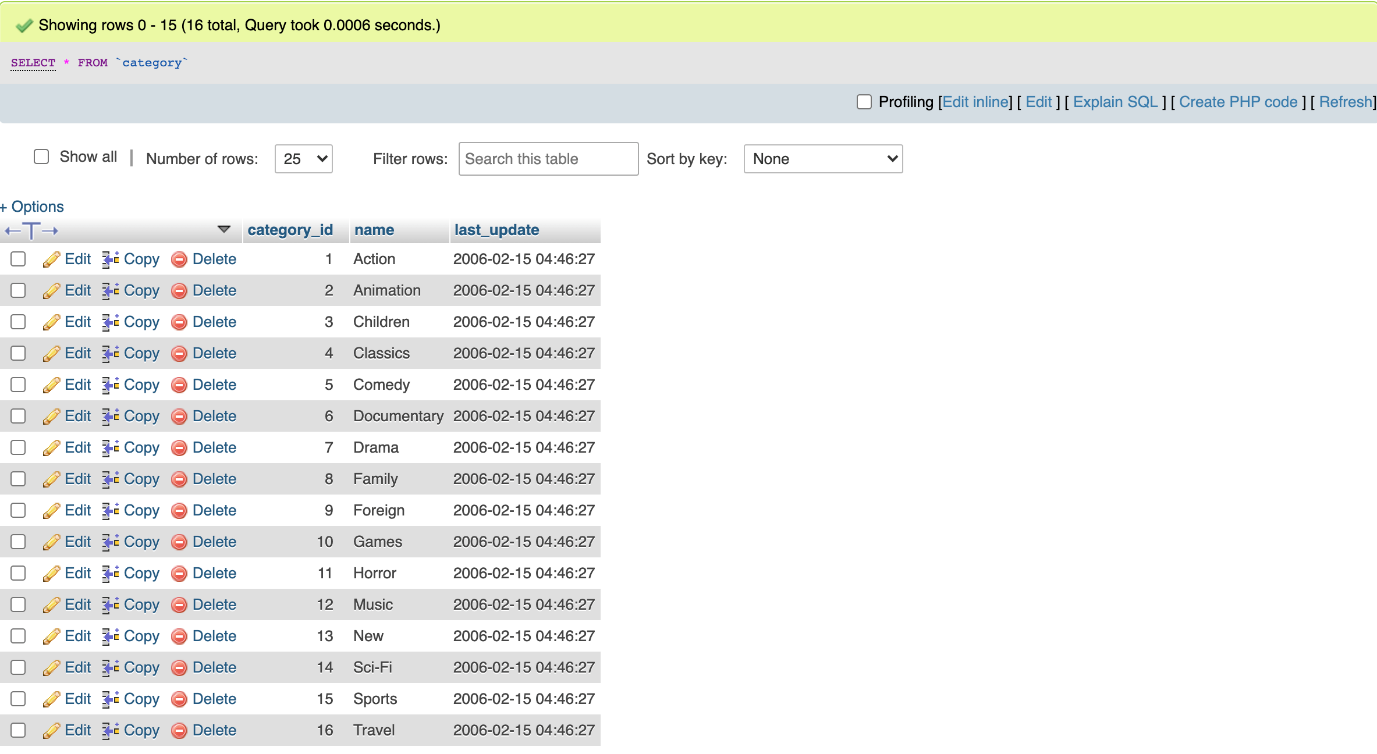
\includegraphics[width=\textwidth]{category_content}
			\caption{Sample content of the table "Category".}
		\end{figure}
		\begin{figure}[H]
			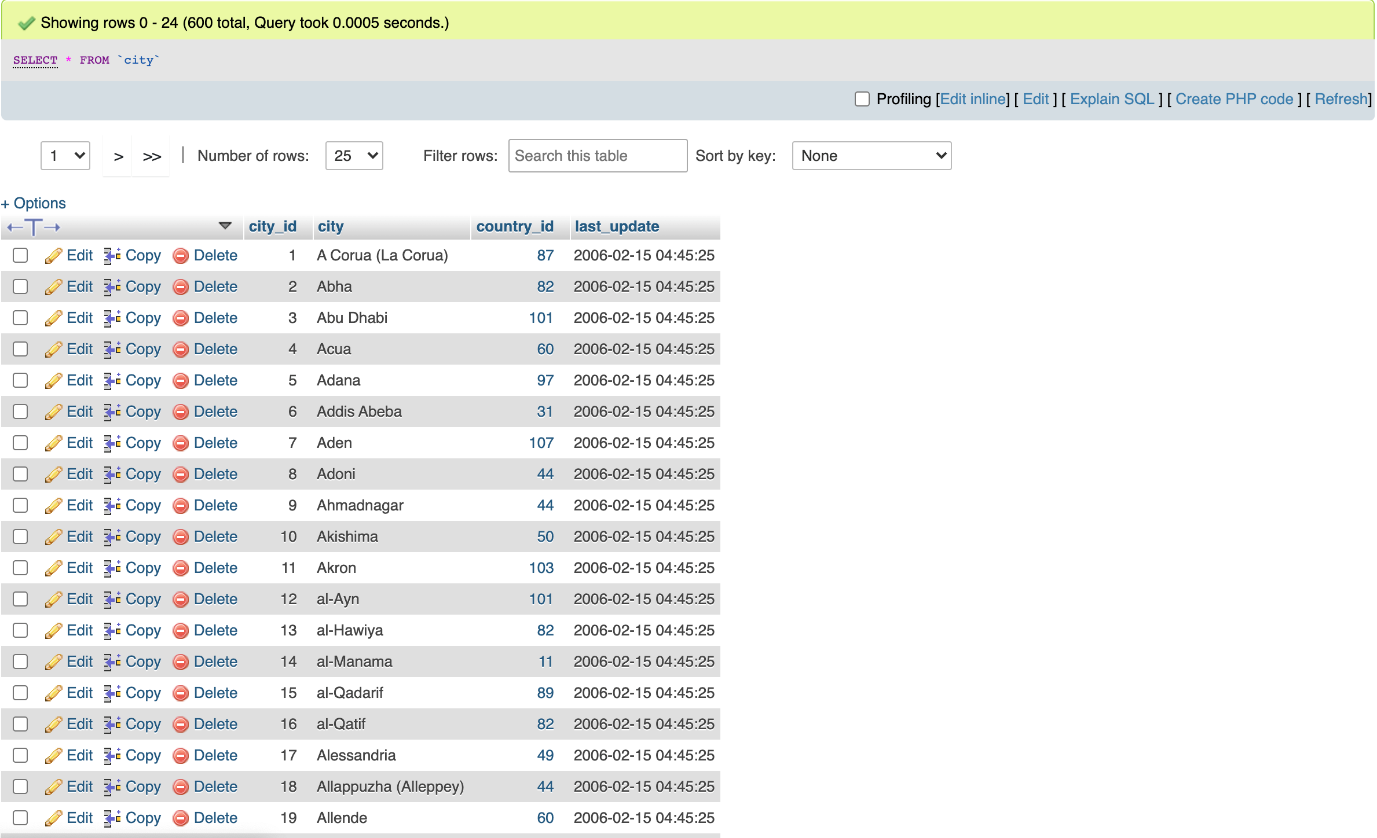
\includegraphics[width=\textwidth]{city_content}
			\caption{Sample content of the table "City".}
		\end{figure}
		\begin{figure}[H]
			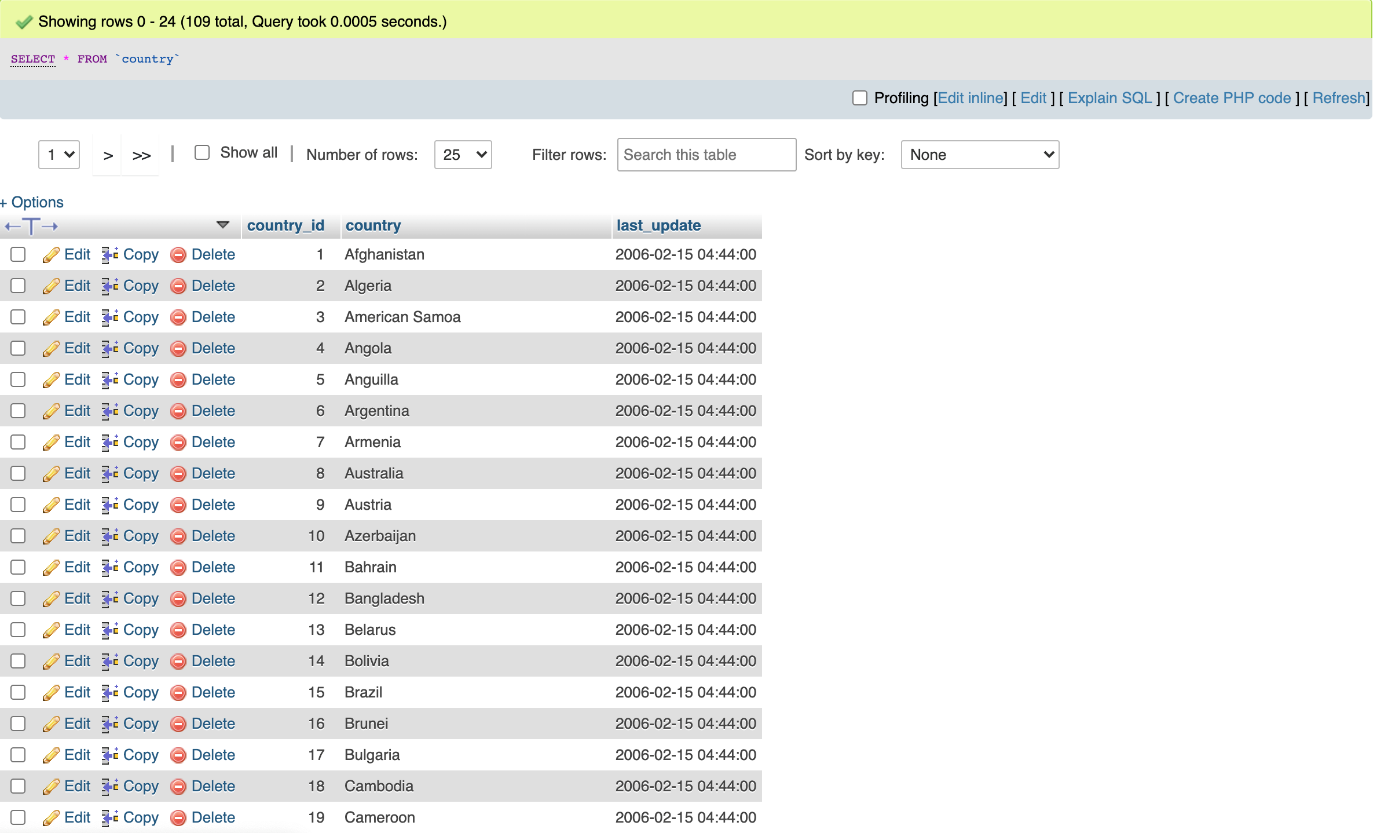
\includegraphics[width=\textwidth]{country_content}
			\caption{Sample content of the table "Country".}
		\end{figure}
		\begin{figure}[H]
			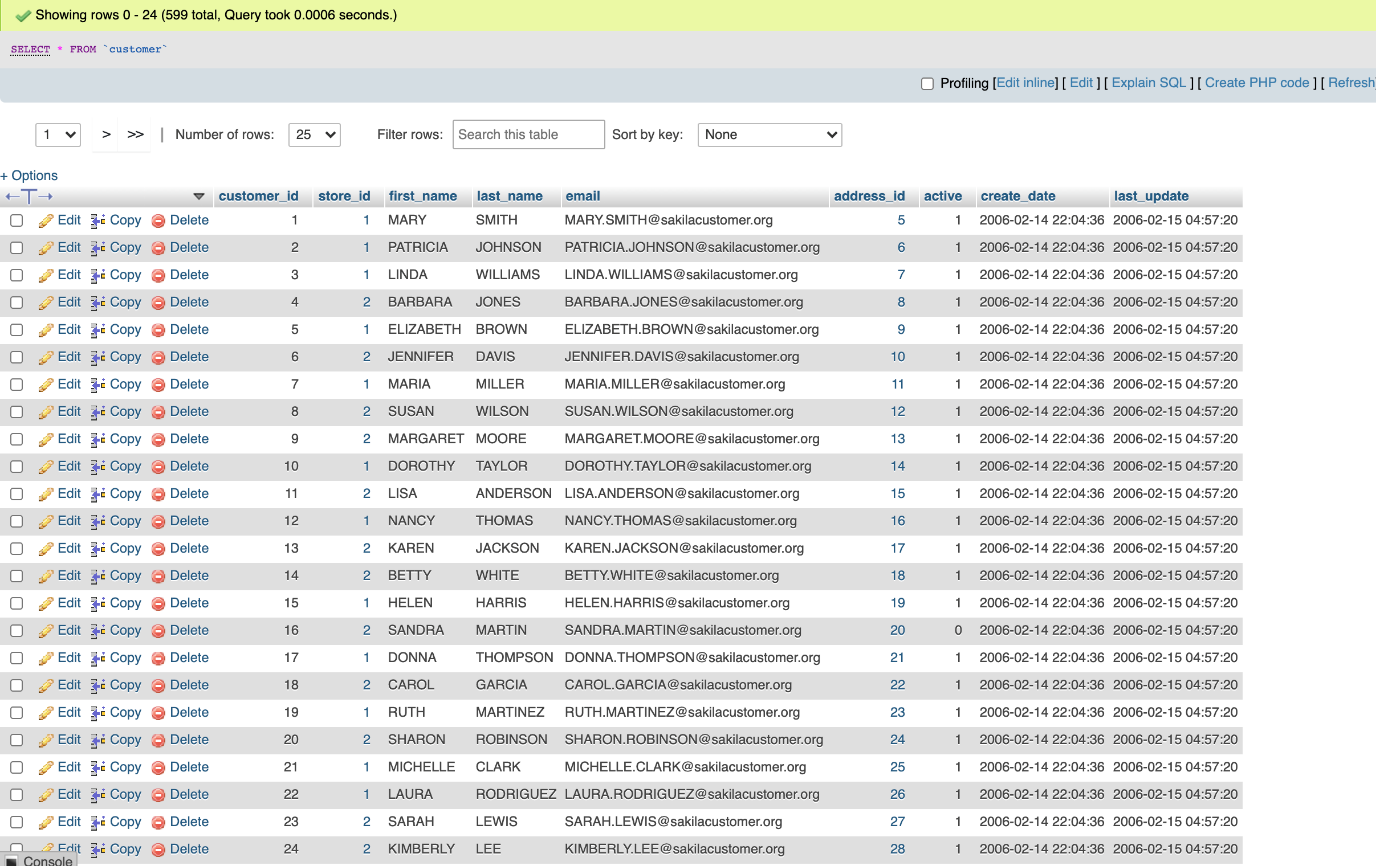
\includegraphics[width=\textwidth]{customer_content}
			\caption{Sample content of the table "Customer".}
		\end{figure}
		\begin{figure}[H]
			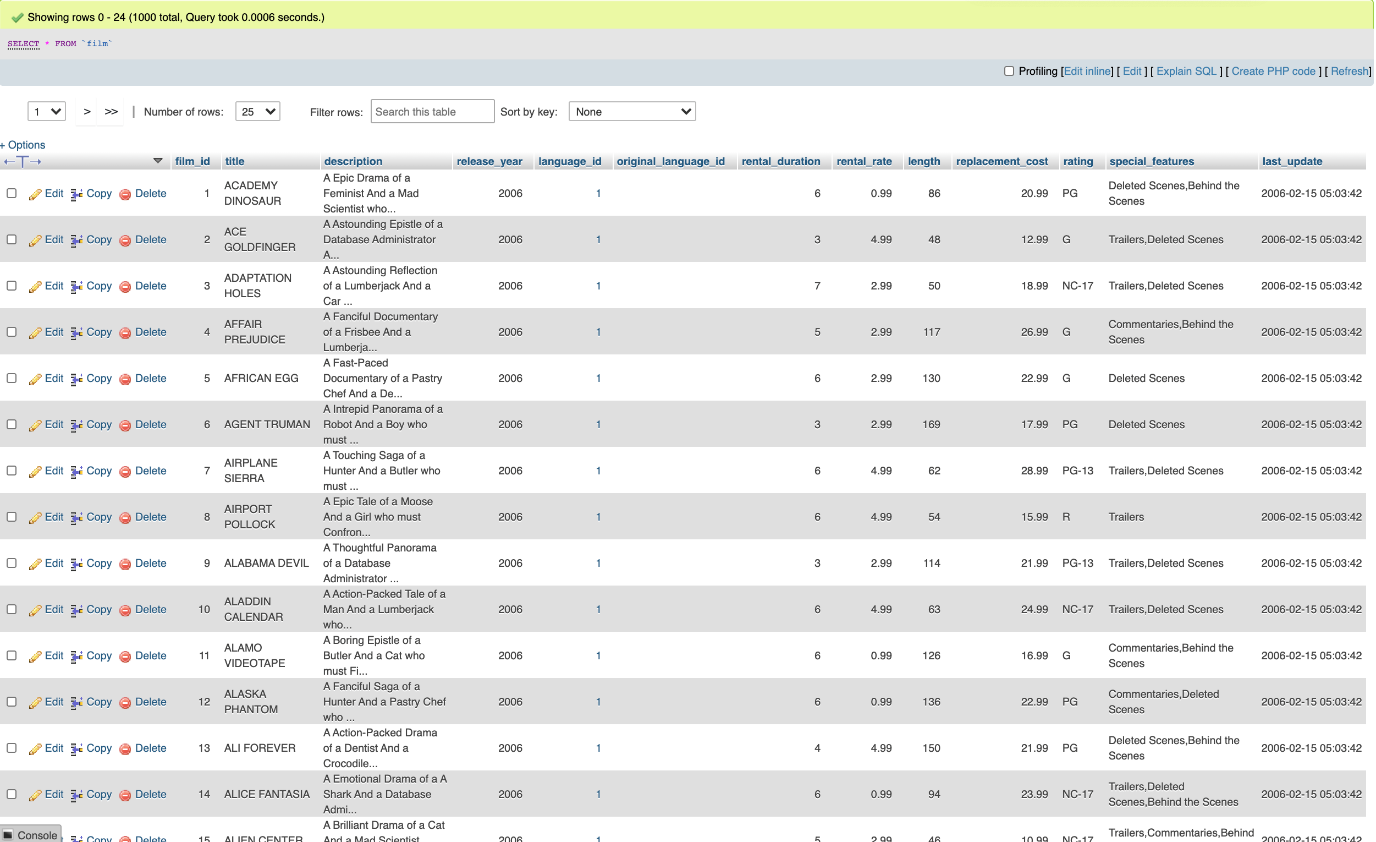
\includegraphics[width=\textwidth]{film_content}
			\caption{Sample content of the table "Film".}
		\end{figure}
		\begin{figure}[H]
			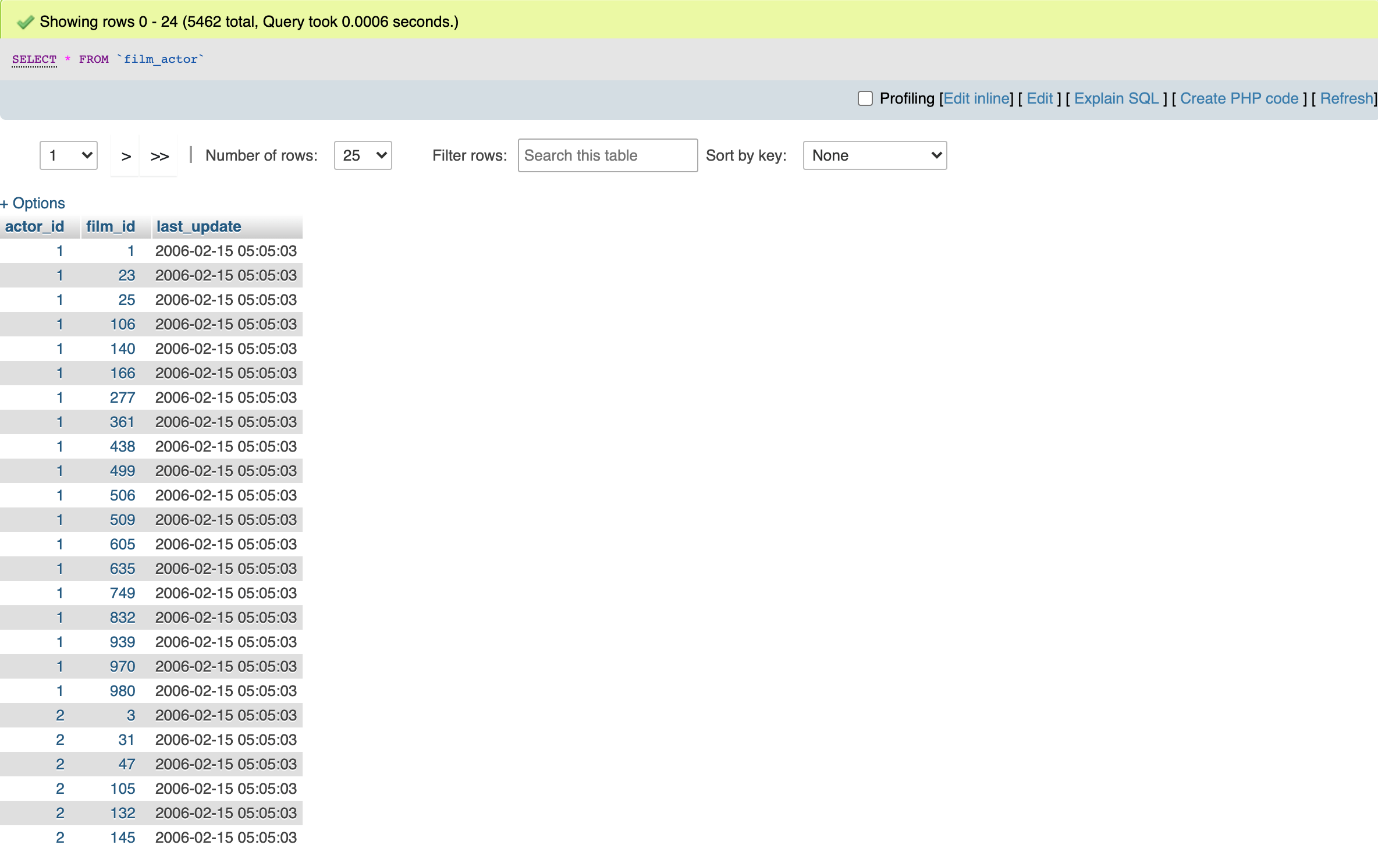
\includegraphics[width=\textwidth]{filmactor_content}
			\caption{Sample content of the table "Film\textunderscore Actor".}
		\end{figure}
		\begin{figure}[H]
			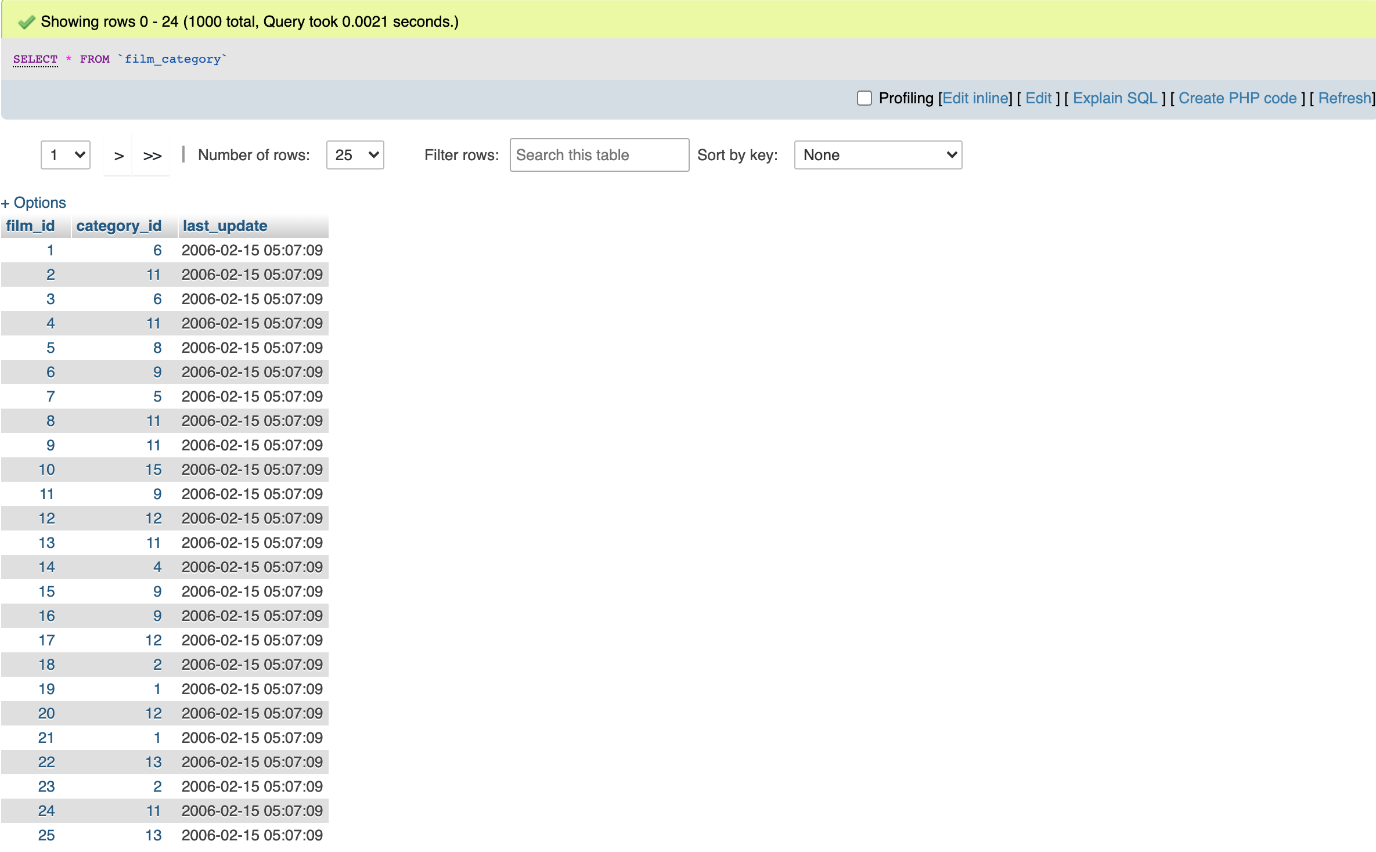
\includegraphics[width=\textwidth]{filmcategory_content}
			\caption{Sample content of the table "Film\textunderscore Category".}
		\end{figure}
		\begin{figure}[H]
			\includegraphics[width=\textwidth]{filmtext_content}
			\caption{Sample content of the table "Film\textunderscore Text".}
		\end{figure}
		\begin{figure}[H]
			\includegraphics[width=\textwidth]{inventory_content}
			\caption{Sample content of the table "Inventory".}
		\end{figure}
		\begin{figure}[H]
			\includegraphics[width=\textwidth]{language_content}
			\caption{Sample content of the table "Language".}
		\end{figure}
		\begin{figure}[H]
			\includegraphics[width=\textwidth]{payment_content}
			\caption{Sample content of the table "Payment".}
		\end{figure}
		\begin{figure}[H]
			\includegraphics[width=\textwidth]{rental_content}
			\caption{Sample content of the table "Rental".}
		\end{figure}
		\begin{figure}[H]
			\includegraphics[width=\textwidth]{staff_content}
			\caption{Sample content of the table "Staff".}
		\end{figure}
		\begin{figure}[H]
			\includegraphics[width=\textwidth]{store_content}
			\caption{Sample content of the table "Store".}
		\end{figure}

\section{Normalization}
	\subsection{Entity Relation Diagram After Normalization}
		\begin{figure}[H]
			\includegraphics[width=\textwidth]{er_normalized}
			\caption{Database structure after normalization.}
		\end{figure}

	\subsection{Tables Affected by Normalization}
		The tables Film\textunderscore Special\textunderscore Features and Special\textunderscore Features are normalized from the Film table to preserve compliance with the First Normal Form. 
		\begin{figure}[H]
			\includegraphics[width=\textwidth]{table_filmspecialfeatures_norm}
			\caption{Table "Film\textunderscore Special\textunderscore Features", normalized.}
		\end{figure}
		\begin{figure}[H]
			\includegraphics[width=\textwidth]{table_specialfeatures_norm}
			\caption{Table "Special\textunderscore Features", normalized.}
		\end{figure}

		The District, City and Address tables have been recompiled after normalization. ////
		The field last_update is retained for the purpose of easing maintenance of the altered tables. ////
		It can be noted that for the Address and City tables, many errors within the database have been uncovered due to the use of normalization that otherwise would have gone unnoticed.  Errors found include: 
		\begin{itemize}
			\item Cities with ID 121, 493 and 583 not having a listed district. Their district_id fields in the newly reorganized City table have been left blank.
			\item Entry with city_id 313 in the City table not existing within the address table. district_id field of this city also left blank in the City table.
			\item Multiple occurences of the same city_id being in multiple districts in the address table. To preserve database integrity after normalization, one of the extra districts is removed with the use of an SQL command containing the GROUP BY keyword. 
		\end{itemize}
		\begin{figure}[H]
			\includegraphics[width=\textwidth]{table_district_norm}
			\caption{Table "District", normalized.}
		\end{figure}
		\begin{figure}[H]
			\includegraphics[width=\textwidth]{table_address_norm}
			\caption{Table "Address", normalized.}
		\end{figure}
		\begin{figure}[H]
			\includegraphics[width=\textwidth]{table_city_norm}
			\caption{Table "City", normalized.}
		\end{figure}
		\begin{figure}[H]
			\includegraphics[width=\textwidth]{table_film_norm}
			\caption{Table "Film", normalized.}
		\end{figure}
		\begin{figure}[H]
			\includegraphics[height = 20cm]{table_filmrental_norm}
			\caption{Table "Film\textunderscore Rental", normalized.}
		\end{figure}
		\begin{figure}[H]
			\includegraphics[width=\textwidth]{table_staff_norm}
			\caption{Table "Staff", normalized.}
		\end{figure}
		\begin{figure}[H]
			\includegraphics[width=\textwidth]{table_stafflogin_norm}
			\caption{Table "Staff\textunderscore Login", newly created after normalization.}
		\end{figure}


	\subsection{Table Structures After Normalization}
		\begin{figure}[H]
			\includegraphics[width=\textwidth]{table_filmspecialfeatures_nstruct}
			\caption{Structure of table "Film\textunderscore Special\textunderscore Features", normalized.}
		\end{figure}
		\begin{figure}[H]
			\includegraphics[width=\textwidth]{table_specialfeatures_nstruct}
			\caption{Structure of table "Special\textunderscore Features", normalized.}
		\end{figure}
		\begin{figure}[H]
			\includegraphics[width=\textwidth]{table_district_nstruct}
			\caption{Structure of table "District", normalized.}
		\end{figure}
		\begin{figure}[H]
			\includegraphics[width=\textwidth]{table_address_nstruct}
			\caption{Structure of table "Address", normalized.}
		\end{figure}
		\begin{figure}[H]
			\includegraphics[width=\textwidth]{table_city_nstruct}
			\caption{Structure of table "City", normalized.}
		\end{figure}
		\begin{figure}[H]
			\includegraphics[width=\textwidth]{table_film_nstruct}
			\caption{Structure of table "Film", normalized.}
		\end{figure}
		\begin{figure}[H]
			\includegraphics[width=\textwidth]{table_filmtext_nstruct}
			\caption{Structure of table "Film\textunderscore Text", normalized.}
		\end{figure}
		\begin{figure}[H]
			\includegraphics[width=\textwidth]{table_staff_nstruct}
			\caption{Structure of table "Staff", normalized.}
		\end{figure}
		\begin{figure}[H]
			\includegraphics[width=\textwidth]{table_stafflogin_nstruct}
			\caption{Structure of table "Staff\textunderscore Login", normalized.}
		\end{figure}

	\subsection{Insertion After Normalization}
		\begin{figure}[H]
			\includegraphics[width=\textwidth]{filmspecialfeatures1_insert_norm}
			\includegraphics[width=\textwidth]{filmspecialfeatures2_insert_norm}
			\caption{Insertion of new data into the table "Film\textunderscore Special\textunderscore Features" after normalization}
		\end{figure}
		\begin{figure}[H]
			\includegraphics[width=\textwidth]{specialfeatures_insert_norm}
			\caption{Insertion of new data into the table "Special\textunderscore Features" after normalization}
		\end{figure}
		\begin{figure}[H]
			\includegraphics[width=\textwidth]{district1_insert_norm}
			\includegraphics[width=\textwidth]{district2_insert_norm}
			\caption{Insertion of new data into the table "District" after normalization}
		\end{figure}
		\begin{figure}[H]
			\includegraphics[width=\textwidth]{city1_insert_norm}
			\includegraphics[width=\textwidth]{city2_insert_norm}
			\caption{Insertion of new data into the table "City" after normalization}
		\end{figure}
		\begin{figure}[H]
			\includegraphics[width=\textwidth]{staff1_insert_norm}
			\includegraphics[width=\textwidth]{staff2_insert_norm}
			\caption{Insertion of new data into the table "Staff" after normalization}
		\end{figure}
		\begin{figure}[H]
			\includegraphics[width=\textwidth]{stafflogin1_insert_norm}
			\includegraphics[width=\textwidth]{stafflogin2_insert_norm}
			\caption{Insertion of new data into the table "Staff\textunderscore Login" after normalization}
		\end{figure}

	\subsection{Deletion After Normalization}
		\begin{figure}[H]
			\includegraphics[width=\textwidth]{staff1_delete_norm}
			\includegraphics[width=\textwidth]{staff2_delete_norm}
			\caption{Data deletion from the table "Staff" after normalization}
		\end{figure}
		\begin{figure}[H]
			\includegraphics[width=\textwidth]{stafflogin1_delete_norm}
			\includegraphics[width=\textwidth]{stafflogin2_delete_norm}
			\caption{Data deletion from the table "Staff\textunderscore Login" after normalization}
		\end{figure}

	\subsection{Updates After Normalization}
		\begin{figure}[H]
			\includegraphics[width=\textwidth]{stafflogin1_update_norm}
			\includegraphics[width=\textwidth]{stafflogin2_update_norm}
			\caption{Update on the table "Staff\textunderscore Login" after normalization}
		\end{figure}

\section{Selections Based on Original Database Using the WHERE Keyword} 
		\begin{figure}[H]
			\includegraphics[height = 20cm]{customer_selectwhere}
			\caption{Table "Customer"}
		\end{figure}
		\begin{figure}[H]
			\includegraphics[height = 20cm]{film_selectwhere}
			\caption{Table "Film"}
		\end{figure}
		\begin{figure}[H]
			\includegraphics[height = 20cm]{filmcategory_selectwhere}
			\caption{Table "Film\textunderscore Category"}
		\end{figure}
		\begin{figure}[H]
			\includegraphics[width=\textwidth]{inventory_selectwhere}
			\caption{Table "Inventory"}
		\end{figure}
		\begin{figure}[H]
			\includegraphics[width=\textwidth]{payment_selectwhere}
			\caption{Table "Payment"}
		\end{figure}
\end{document}